%% P1 - AI in Civil Engineering (Springer Nature), Original Article.
%% Plantilla: Springer Nature LaTeX template v3.1 (sn-jnl), opcion sn-apa
%% (citas autor-ano APA, lista alfabetica: guias de AICE, ver JOURNAL.md).
%% Compilar: pdflatex main && bibtex main && pdflatex main && pdflatex main
%%
%% Estado (03/10/2026): Related Work, Method, Results, Discussion y
%% Limitations redactados con los resultados nuevos de F1. Introduccion,
%% Conclusion y Abstract se escriben despues (guia metodologica 2.8: el
%% abstract al final). Toda cifra de resultados sale de results/; las que aun
%% no existen van marcadas con \pend{...}, que se imprime en rojo.
%% Autoria NO decidida: marcador [Author list pending] (PLAN_AICE.md, sec. 1).

\documentclass[pdflatex,sn-apa]{sn-jnl}

\usepackage{graphicx}
\usepackage{multirow}
\usepackage{amsmath,amssymb,amsfonts}
\usepackage{booktabs}
\usepackage{xcolor}
\usepackage{textcomp}
\usepackage[title]{appendix}

% Marcador de cifra pendiente de resultados (se elimina antes del envio;
% verificar_envio.py lo detecta).
\newcommand{\pend}[1]{\textcolor{red}{[\textbf{PENDING:} #1]}}

\raggedbottom

% APA 7 (guias de AICE) frente a apacite, que sigue APA 6:
% - sin "Retrieved from" delante de la URL;
% - "et al." desde la primera cita con tres o mas autores (\shortcites, lista
%   generada desde refs.bib); la lista de referencias admite hasta 20 autores
%   (cambio anotado en sn-apacite.bst).
\AtBeginDocument{\renewcommand{\BRetrievedFrom}{}}

\begin{document}

\shortcites{lipton2014,miller2021,santos2022,abeysuriya2026,fountoukidou2024,dorafshan2018sdnet,maguire2018sdnetdata,cha2017,dorafshan2018comparison,alipour2019,rashid2025,zhu2026concracknet,yang2020crack500,spencer2019,zhou2023dg,geirhos2020,kumar2022,kornblith2019,bouthillier2021,he2016,howard2019,dosovitskiy2021,steiner2021}

\title[Cross-domain generalization of concrete crack classifiers]{Cross-Domain Generalization of Concrete Crack Classifiers: A Transfer Matrix Across Surfaces and Capture Campaigns}

%% Autoria pendiente de decision: no se escriben nombres, orden ni ORCID.
\author{\fnm{[Author list pending]}}
\affil{\orgname{[Affiliation pending]}}

\abstract{Concrete crack classifiers have reported over 95\% accuracy on held-out splits of their own collection, which says little about a new site. We fine-tuned four ImageNet-pretrained architectures on each of four image domains, the bridge-deck, pavement and wall subsets of SDNET2018 and an independent collection from the Middle East Technical University (METU), with three seeds, testing each model on all four. On the balanced test sets, labeling every patch as cracked gives an F1 score of 0.667. F1 averaged 0.824 within SDNET2018 subsets, 0.998 within METU and 0.654 between SDNET2018 surfaces. Transfer between collections was asymmetric: 0.782 from SDNET2018 to METU and 0.437 in the reverse direction. Part of this gap reflects an easy METU target, but METU-trained models lost most relative to either the source or the target diagonal. Of 144 out-of-domain results, 78 scored at or below the F1 of the always-crack classifier, almost all by missing cracks, though all exceeded chance in balanced accuracy. From METU to SDNET2018 the area under the receiver operating characteristic curve was 0.70, and a threshold chosen on 50 labeled target patches raised balanced accuracy only from 0.63 to 0.66. The loss did not grow with architecture size and was not significantly reduced by aggressive augmentation, histogram equalization or random rescaling. It also appeared in a linear classifier on frozen features and persisted, reduced, under a photo-grouped split. Before a crack classifier informs maintenance decisions at a new site, its precision and recall should be measured on labeled images from that site.}

\keywords{Concrete crack classification, Domain shift, Cross-dataset evaluation, Transfer learning, Infrastructure inspection, SDNET2018}

\maketitle

% =====================================================================
\section{Introduction}\label{sec:intro}

A crack classifier trained on an agency's own bridge-deck photographs and reported at 98\% accuracy on a held-out split describes how well the model has learned that set of photographs. Before relying on it, the agency needs to know how the model performs on structures photographed by different crews and equipment, which a held-out split of its own photographs cannot show.

Within-collection figures are high: \citet{cha2017} reached about 98\% accuracy on 40,000 concrete patches; the authors of SDNET2018 benchmarked AlexNet at 87.5--95.5\% accuracy within each of its subsets \citep{dorafshan2018sdnet}; \citet{ozgenel2018} reported 0.99 on a held-out split of the collection from the Middle East Technical University (METU). In each case the test patches come from the same collection as the training patches, and when patches are cut from larger photographs and split at random, from the same photographs \citep{kapoor2023, abeysuriya2026}. A held-out score of this kind predicts field performance only if the test set represents the conditions of use and is independent of the training data \citep{hasan2025}.

Whether a test set meets that condition depends on how the collection was assembled. \citet{torralba2011} showed that object-recognition datasets carry a signature strong enough for a classifier to tell them apart, and measured the cost by training on each dataset and testing on all the others. In civil engineering, a systematic review of 46 deep-learning studies of post-earthquake damage assessment found weak evidence that the reported models generalize to unseen data and asked for cross-dataset testing \citep{abeysuriya2026}, and work on concrete bridge defects in this journal lists cross-bridge and cross-site evaluation as an open step \citep{lateef2026}.

Cross-dataset tests of crack classifiers do exist \citep{ozgenel2018, rashid2025}, and domain adaptation has been used to recover part of the loss with images of the target site \citep{santos2022, zhu2026concracknet}. A shift between two crack datasets mixes a change of surface with a change of capture campaign (camera, distance, site and country), and we found no study that measures the two apart. The two directions of a dataset pair have not been compared with replicated runs and a test of their difference, nor read against the score of a trivial classifier. It is also not known whether the loss is created by fine-tuning on the source or is already present in the pretrained features, or whether training on several sources helps when the total amount of data is held fixed.

This paper measures those quantities with a 4$\times$4 transfer matrix. Three subsets of SDNET2018, bridge decks, pavements and walls, were photographed by one research group with the same camera at the same working distance, the decks in a laboratory and the walls and pavements on a university campus; the METU collection comes from another country, camera and team. Every domain is reduced to the same size and class balance, so that a classifier labeling every patch as cracked scores 0.667 on every test set in the F1 score of the crack class, the harmonic mean of its precision and recall. Four ImageNet-pretrained architectures, from 1.5 to 11.2 million parameters, are fine-tuned on each domain with three seeds and deterministic training, and tested on all four; the same design is repeated with three training-time interventions, the third, random rescaling, added to test an explanation of the first results, with a linear probe on frozen features and with three source domains at the data budget of one. Every cell records precision and recall as well as F1, and a split grouped by parent photograph tests whether leakage between patches drives the results.

The study makes four contributions:
\begin{enumerate}
\item A transfer matrix that separates cross-surface from cross-campaign transfer and reports the two cross-campaign directions apart. They differ by 0.345 F1 (0.782 against 0.437) with the training run as unit, and by 0.265 under a split grouped by photograph. Pooled, as the analysis fixed before the first runs did, the two directions show no difference from cross-surface transfer. Part of the difference reflects that METU is an easy target, but transfer from METU to SDNET2018 loses most whether the loss is measured from the source or the target diagonal.
\item The failure mode of out-of-domain models: 77 of the 144 off-diagonal cells score below the F1 of the always-crack classifier and one equals it, although all are better than chance in balanced accuracy, and 77 of these 78 keep precision above recall, so their errors are mostly missed cracks. From METU to SDNET2018 the models also rank target patches weakly, and a threshold chosen on 50 target labels changes balanced accuracy little.
\item Tests of where the loss comes from. Architecture changes the relative drop by at most 0.165 within a partition, against at least 0.456 across partitions. None of three training-time interventions reduces the loss significantly; the effect of random rescaling, which targets a difference in how the two collections frame cracks, is inconclusive and leaves the ranking of target patches unchanged. A linear probe on frozen ImageNet features fails in the same way from METU to SDNET2018, so for these models the loss is not created by fine-tuning. Three sources at the budget of one do not differ from the best single source.
\item Recommendations for validating a crack classifier at a new site, derived from the results above (Sections~\ref{sec:disc-implications} and~\ref{sec:conclusion}).
\end{enumerate}

% =====================================================================
\section{Related work}\label{sec:related}

\subsection{High accuracy within one image collection}\label{sec:related-crack}

Image-based crack classification reached high accuracy early. \citet{cha2017} trained a convolutional network on 40,000 concrete patches of 256$\times$256 pixels and reported about 98\% accuracy; they also ran the network as a sliding window over 55 larger photographs of a structure not used for training and compared it with Canny and Sobel edge detection. \citet{dorafshan2018comparison} compared six edge detectors with AlexNet on 19 high-definition concrete photographs split into 3,420 patches, 319 of them cracked, and the network labeled patches with 99\% accuracy, a figure that a model labeling every patch as uncracked would already bring to about 91\%. The same group released SDNET2018, more than 56,000 patches of bridge decks, walls and pavements, and benchmarked AlexNet within each subset at 87.5--95.5\% accuracy \citep{dorafshan2018sdnet}. \citet{alipour2019} moved from patch labels to pixel-level segmentation with fully convolutional networks. In these studies the headline figure describes the collection the model was trained on: the same cameras and sites and, when patches are cut from larger photographs and split at random, patches of the same photographs.

\citet{ozgenel2018} measured what happens outside that collection. They fine-tuned seven ImageNet-pretrained networks on 40,000 patches cut from photographs of campus buildings, the collection later published as METU \citep{ozgenel2019metu}, and tested each network on a held-out split and on three test sets from other sites: concrete pavements, concrete walls of other buildings and brickwork. The best accuracy of VGG16 on the three external sets was 0.96 to 0.98, while ResNet101 and ResNet152 scored 0.99 on the held-out split and 0.54 to 0.77 outside it, which the authors attributed to overfitting by the residual networks. \citet{rashid2025} extended the comparison to a full cross-testing design: four models trained on each of six public crack datasets, including SDNET2018 and the METU collection (listed there under another name), and tested on all the others. Accuracy fell for most pairs once the test set came from another dataset, and the authors concluded that flips and small rotations do not cover the variation between datasets. Each configuration was run once, SDNET2018 entered the matrix as a single dataset, and class balance and dataset size differed between datasets; we return to what their matrix shows about the two directions in Section~\ref{sec:disc-direction}.

The same gap appears in neighboring tasks reported in this journal. \citet{lateef2026} classified co-occurring defects on a public multi-label dataset of concrete bridge images and found that every model lost accuracy on a synthetic test set generated from the same images; their future work asks for cross-bridge and cross-site evaluation. A systematic review of 46 deep-learning studies of element-level damage after earthquakes found weak evidence of generalization to unseen data and asked for cross-dataset and cross-event testing \citep{abeysuriya2026}. It also warned that patches cut from one parent image and split between training and test sets leak information, a point that matters for both collections used here (Section~\ref{sec:prep}).

\subsection{Dataset bias and distribution shift}\label{sec:related-shift}

\citet{torralba2011} showed for object recognition that classifiers can identify which collection an image came from, and reported the consequence as a matrix: train on one dataset, test on all, and compare each row with its own diagonal. We apply the same design to images of concrete surfaces. \citet{geirhos2020} describe the mechanism behind such losses as shortcut learning, decision rules that solve the test set drawn from the training distribution but fail under a shift. Two of their examples are analogous to the crack setting: a pneumonia classifier that worked in the hospitals it was trained on and failed in new ones, and a toy task in which a network trained on images of stars and moons learned the position of the object, which was correlated with its class during training, and failed when position was varied at test time.

Two families of methods respond to distribution shift. Domain adaptation aligns source and target distributions and therefore needs target data during training \citep{wang2018}. For crack images, \citet{santos2022}, in this journal, trained a classifier on the METU collection and tested it on patches from a concrete dam: accuracy fell from above 99\% to 54\%, and adversarial adaptation with unlabeled dam patches raised it to 84\%. \citet{zhu2026concracknet} adapted classifiers with pseudo-labels in six cross-domain scenarios built from SDNET2018 and reported above 95\% accuracy in each, and \citet{chun2024} adapted a crack segmentation model to a new site with as few as 100 target images. Domain generalization asks for a model that works on an unseen target without any of its data, and is usually evaluated by holding out one domain at a time \citep{zhou2023dg}. Under careful model selection, standard training on the pooled sources matches most algorithms designed for it \citep{gulrajani2021}. A separate question is how much of a pretrained network to fine-tune. Fine-tuning all layers and training a linear classifier on frozen features are the two standard regimes \citep{kornblith2019}; \citet{kumar2022} found that fine-tuning wins in distribution but can lose out of distribution when the pretrained features are good and the shift is large.

These comparisons also depend on how training and test samples are separated. \citet{kapoor2023} list non-independence between training and test samples, for instance samples from the same unit on both sides of the split, among the forms of leakage that inflate reported performance. \citet{fountoukidou2024} split their synthetic bridge images by bridge for that reason, and traced part of their synthetic-to-real gap to viewing distance, close-ups against overall views. \citet{bouthillier2021} showed that variation from data sampling and initialization can be large enough to dominate the differences between the methods being compared.

\subsection{Transfer between civil structures}\label{sec:related-civil}

The same problem arises in vibration-based structural health monitoring. \citet{luleci2023} trained a generative model on the healthy and damaged states of a numerical model of one prestressed bridge and used it, without any data from the target, to translate the state of a structurally different bridge, framing the task as domain generalization. They leave open how similar two structures must be for such transfer to work. Inspection by computer vision is reviewed by \citet{spencer2019}, whose goal for these systems is to turn images into information that inspection decisions can rely on.

\subsection{Gap addressed}\label{sec:gap}

Existing cross-dataset tests of crack classifiers \citep{ozgenel2018, rashid2025} confound a change of surface with a change of capture campaign. They also compare the two directions of a campaign pair without replicated runs or a test of the difference, and do not report the score of a trivial classifier on the same test sets. Several of the remaining questions have general answers outside crack classification, for linear probing \citep{kumar2022}, pooled sources \citep{gulrajani2021} and leakage \citep{kapoor2023}; whether they hold for crack images has not been measured. We address these points on two public collections.

% =====================================================================
\section{Method}\label{sec:method}

Figure~\ref{fig:pipeline} summarizes the pipeline. The baseline matrix was first run in an earlier, unpublished version of this study, without deterministic training, and the split of cross-campaign transfer by direction (Section~\ref{sec:matrix}) was introduced after those runs. Every run reported here comes from a complete retraining, deterministic this time and therefore not a bit-for-bit copy of the earlier runs, whose design and statistical tests were fixed before it started. The directional result was exploratory when first observed and is retested here on new runs of the same collections and code; it is not an independent replication.

\begin{figure}[t]
\centering
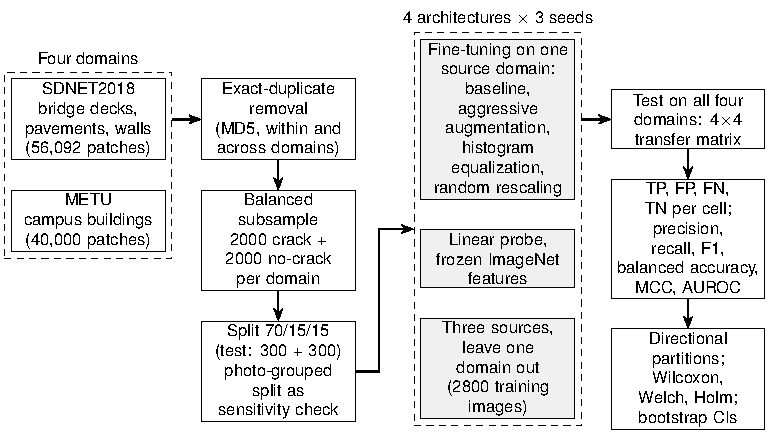
\includegraphics{fig_pipeline.pdf}
\caption{Experimental pipeline. Four domains are deduplicated, subsampled to the same size and class balance, and split; each architecture is then trained under three regimes (fine-tuning on one source domain, as a baseline and with three training-time interventions; linear probe on frozen features; three-source training with one domain held out) and every model is tested on the test split of all four domains. TP, FP, FN and TN are true and false positives and negatives; MCC, Matthews correlation coefficient; AUROC, area under the receiver operating characteristic curve; CI, confidence interval}\label{fig:pipeline}
\end{figure}

\subsection{Datasets and domains}\label{sec:data}

We use four image domains. Three are the subsets of SDNET2018 \citep{dorafshan2018sdnet, maguire2018sdnetdata}: bridge decks (SDNET-Deck, 13,620 patches, 14.9\% cracked), pavements (SDNET-Pavement, 24,334 patches, 10.7\% cracked) and walls (SDNET-Wall, 18,138 patches, 21.2\% cracked). The dataset authors photographed each surface with a 16-megapixel camera at a working distance of 500~mm and cut each photograph into 256$\times$256 patches covering about 60$\times$60~mm; the deck images were taken in a laboratory on stored full-scale bridge-deck sections, and the wall and pavement images on the university campus \citep{dorafshan2018sdnet}. Patch file names keep the identifier of the parent photograph and number its patches from 1 to 252 (1 to 234 for pavements): SDNET-Deck comes from 54 photographs, SDNET-Pavement from 104 and SDNET-Wall from 72. The three subsets share camera, working distance and research group; they differ in the surface photographed and, for the decks, in the site.

The fourth domain is the METU collection \citep{ozgenel2019metu}: 40,000 patches of 227$\times$227 pixels, half of them cracked, cut from high-resolution photographs of walls and floors of buildings on the campus of Middle East Technical University (458 photographs of 4032$\times$3024 pixels according to the dataset record, 500 according to \citealp{ozgenel2018}). The photographs were taken about one meter from the surface with the camera perpendicular to it, on the same day and under similar illumination \citep{ozgenel2018}. The cracked patches are close-ups in which the crack is centered in the patch \citep{santos2022}. METU file names carry no photograph identifier. Pairing METU with an SDNET2018 subset changes the capture campaign: camera, distance, site and country.

\subsection{Preprocessing and splits}\label{sec:prep}

We removed exact duplicates by their MD5 checksum over all 96,092 files before any sampling: 1,611 duplicates within domains and none across domains. Two properties of the raw collections would otherwise confound the matrix. The class prior ranges from 10.7\% to 50\% cracked, so a model trained on METU and tested on SDNET2018 would face a change of prior on top of the change of domain; and the domains differ in size by a factor of nearly three. We therefore subsampled every domain to 2,000 cracked and 2,000 uncracked patches, the largest balanced sample the smallest class allows (2,022 cracked SDNET-Deck patches after deduplication). This equalises class prior and training-set size across domains, so a difference between rows of the transfer matrix reflects the source domain and not the amount or balance of its data. It also limits each model to 2,800 training patches, which may keep within-domain F1 below what training on the full collections would reach (Section~\ref{sec:limitations}).

Each domain was split 70/15/15 into training, validation and test sets, stratified by class: 2,800, 600 and 600 patches, with exactly 300 cracked and 300 uncracked patches in every test set. A classifier that labels every patch as cracked therefore scores precision 0.5, recall 1.0 and F1 $=2/3\approx0.667$ on every test set; we report out-of-domain F1 against this value. All patches were resized to 224$\times$224 pixels.

The split was drawn at patch level, so patches cut from the same photograph fall on both sides of it. In the three SDNET2018 subsets every test patch shares its parent photograph with training patches. This is the non-independence that \citet{kapoor2023} classify as leakage, and it can only inflate the diagonal of the matrix: off-diagonal cells compare different collections, which share no photographs. To measure its effect we built a second split of the same patches grouped by parent photograph for the SDNET2018 subsets, with test and validation sets again of exactly 300 + 300 patches (8, 16 and 11 photographs in the SDNET-Deck, -Pavement and -Wall test sets) and 1,390 training patches per class, equal across the three subsets. METU keeps its original split because its file names do not identify the photograph. We retrained the baseline condition under this split as a sensitivity analysis (Section~\ref{sec:res-sensitivity}).

\subsection{Architectures and training}\label{sec:train}

We compared four ImageNet-pretrained architectures from the PyTorch Image Models (timm) library (Table~\ref{tab:arch}): ResNet-18 \citep{he2016}, EfficientNet-B0 \citep{tan2019}, MobileNetV3-Small \citep{howard2019} and ViT-Tiny with 16-pixel patches, a vision transformer (ViT) \citep{dosovitskiy2021} whose configuration and weights come from the release of \citet{steiner2021}. They span three convolutional neural network (CNN) designs and a transformer, and 1.52 to 11.18 million parameters.

\begin{table}[t]
\caption{Architectures compared. Parameters counted with the two-class head; probe dimension is the size of the frozen feature used by the linear probe (Section~\ref{sec:probe})}\label{tab:arch}
\begin{tabular*}{\textwidth}{@{\extracolsep\fill}llrr@{}}
\toprule
Architecture & Family & Parameters (M) & Probe dim. \\
\midrule
ResNet-18 & CNN, residual & 11.18 & 512 \\
EfficientNet-B0 & CNN, compound scaling & 4.01 & 1280 \\
MobileNetV3-Small & CNN, architecture search & 1.52 & 1024 \\
ViT-Tiny/16 & Vision transformer & 5.52 & 192 \\
\botrule
\end{tabular*}
\footnotetext{Input 224$\times$224 pixels and batch size 64 for all four. timm weight tags: \texttt{resnet18.a1\_in1k}, \texttt{efficientnet\_b0.ra\_in1k}, \texttt{mobilenetv3\_small\_100.lamb\_in1k}, \texttt{vit\_tiny\_patch16\_224.augreg\_in21k\_ft\_in1k}.}
% Origen de la tabla: results/tables/tabla_arquitecturas.csv (src/tabla_arquitecturas.py).
\end{table}

All four were fine-tuned with the same settings: the AdamW optimizer, Adam with decoupled weight decay \citep{loshchilov2019} (learning rate $3\times10^{-4}$, weight decay $10^{-4}$), cosine annealing over at most 12 epochs, cross-entropy loss, mixed precision and batch size 64. Training images were flipped horizontally at random and every image was normalized with the ImageNet channel statistics. Training stopped when the F1 of the crack class on the source validation set had not improved for 3 epochs, and the weights of the best epoch were kept. We used no per-architecture tuning, so the comparison holds the training recipe fixed.

Training was deterministic: every run fixed the seeds of Python, NumPy and PyTorch, enabled PyTorch's deterministic algorithms with a fixed workspace for NVIDIA's cuBLAS linear-algebra library, disabled the autotuner of its cuDNN library, and drew the order of training batches from a seeded generator. In a pilot, two runs of the same configuration (ResNet-18, seed 42, four source domains) produced identical predictions for all 9,600 test images they scored and identical training losses at every epoch. We used PyTorch 2.13, timm 1.0.28 and CUDA 12.6 on one NVIDIA RTX 4050 Laptop graphics processing unit with 6~GB of memory. Evaluation also ran in mixed precision: in 67 of the 806,400 test predictions reported in this paper, almost all from EfficientNet-B0, the half-precision forward pass returned a non-finite output, and these patches were counted as uncracked. Counting them as correct or as wrong instead changes no cell by more than 0.025 F1 (0.007 outside the scale intervention of Section~\ref{sec:interventions}), and none of the affected cells has a METU source.

\subsection{Transfer matrix and directional partitions}\label{sec:matrix}

For each architecture and seed we trained one model on each of the four domains and tested it on the test sets of all four, giving a 4$\times$4 matrix of crack-class F1. With three seeds (42, 43, 44) this is 48 training runs and 192 cells per condition. The a priori hypothesis was that within-domain F1 would exceed 0.97 in every domain, that the loss would be moderate between surfaces, larger between campaigns, and larger for larger architectures.

We group the off-diagonal cells into three directional partitions. Cross-surface cells pair two SDNET2018 subsets; they share a campaign by construction and serve as the control, the cost of a change of surface alone. The cross-campaign cells split into SDNET2018-to-METU and METU-to-SDNET2018. The a priori analysis used a single cross-campaign category; we report both directions because pooling them can hide a difference between them.

\subsection{Training-time interventions}\label{sec:interventions}

Three interventions were run for all 48 combinations and compared with the baseline. None uses any target data. Aggressive augmentation added random rotation up to 30$^\circ$, color jitter (brightness and contrast 0.4, saturation 0.2), random translation up to 10\% and additive Gaussian noise ($\sigma=0.05$ after normalization) to the training images only. Histogram equalization was applied per color channel to training, validation and test images alike: it normalizes appearance rather than augmenting it, and applying it to training images only would add a mismatch between training and evaluation inside every domain.

The third intervention, scale augmentation, was added after the other results were known, to test the explanation that METU-trained models fail on SDNET2018 because the two collections frame cracks differently (Section~\ref{sec:disc-diagonal}). Each training image, already resized to 224$\times$224 pixels, was rescaled by a factor drawn uniformly between 0.5 and 1.5. Enlarged images were cropped back to 224$\times$224 at a random position; reduced images were padded back to 224$\times$224 by reflection, at a random offset, so that no black border could serve as a new cue. The rescaling therefore also moves the crack within the patch, and with factors near 0.5 the reflection can repeat part of a crack as a mirror image. Horizontal flips followed as in the baseline; validation and test images were not changed. The design, the scale range and the tests (Section~\ref{sec:stats}) were fixed before the first of these runs and not changed afterwards.

\subsection{Linear probe}\label{sec:probe}

To separate what fine-tuning (FT) adapts to the source domain from what the pretrained features already carry, we trained a linear classifier on frozen features, a linear probe (LP). For each architecture and domain we extracted the features of all training, validation and test patches once, with the pretrained network in evaluation mode, no augmentation and the classification head removed (dimensions in Table~\ref{tab:arch}). For each architecture, seed and source domain we then trained a linear layer with two outputs on the source training features with AdamW (learning rate $10^{-3}$, weight decay $10^{-4}$), batches of 256, at most 100 epochs and early stopping after 10 epochs without improvement of validation F1. The seed sets the initialization and the batch order, so the three seeds give three different probes. Each probe was tested on the four test sets, giving the same 4$\times$4 matrix as fine-tuning.

\subsection{Three sources, one domain held out}\label{sec:multisource}

An operator with labeled images from several sites can train on all of them. We tested this with the leave-one-domain-out protocol of domain generalization \citep{zhou2023dg}: for each held-out domain, a model was fine-tuned on the other three and tested on the held-out test set. To separate the effect of source diversity from that of data quantity, the combined training set was subsampled to the size of a single-source training set: 2,800 patches, 934, 933 and 933 from the three sources, 1,400 per class; the combined validation set had 200 patches from each source. The sample was drawn once with seed 42 from the training and validation splits defined above, and the baseline training recipe was used, giving 4 held-out domains $\times$ 4 architectures $\times$ 3 seeds = 48 runs.

\subsection{Statistical analysis}\label{sec:stats}

The primary metric is the F1 score of the crack class, the harmonic mean of its precision and recall. For each cell we also recorded the counts of true positives (TP), false positives (FP), false negatives (FN) and true negatives (TN), precision and recall, and the predicted probability of every test patch. A cell with F1 exactly 2/3 is counted as a tie with the always-crack classifier.

The analysis fixed before the first runs was a two-way analysis of variance (ANOVA) of F1 on architecture (4 levels) and train-test pair (16 levels) with interaction, the three seeds as replicates (192 observations), followed by Tukey's honestly significant difference (HSD) test on the three transfer categories. We report it, with Levene's test of equal variances and the Shapiro-Wilk test of the residuals, but do not base conclusions on it: each model contributes four cells, so the cells are not independent, and both assumption tests fail (Section~\ref{sec:res-direction}).

The directional comparisons use the training run (architecture $\times$ source $\times$ seed) as unit, averaging the cells each run contributes to a partition. Partitions that come from the same runs are compared on paired run means with the Wilcoxon signed-rank test: within-domain, cross-surface and SDNET2018-to-METU transfer for the 36 runs with an SDNET2018 source, and within-domain against METU-to-SDNET2018 transfer for the 12 runs with a METU source. Partitions that come from different runs are compared with Welch's $t$-test \citep{welch1947}. Holm's correction \citep{holm1979} is applied over the six comparisons; effect sizes are the matched-pairs rank-biserial correlation $r$ for paired comparisons and Cliff's $\delta$ \citep{cliff1993} for independent ones. A first version of this analysis applied Welch's test to all six pairs, which treats partitions from the same runs as independent; we report the paired design. Confidence intervals (CI) are percentile bootstrap intervals with 10,000 resamples of training runs; Holm-adjusted $p$ values are written $p_\mathrm{Holm}$. Differences are computed from unrounded values and can differ by 0.001 from the difference of the rounded values shown.

The relative drop of an off-diagonal cell is
\begin{equation}
\Delta = \frac{F_1(s \to s) - F_1(s \to t)}{F_1(s \to s)},\label{eq:drop}
\end{equation}
where $F_1(s\to s)$ is the within-domain F1 of the same model, that is, same architecture, seed and source domain $s$. Anchoring each cell on its own source matters because the four diagonals differ.

For the questions added in this study the tests were fixed before training, all with the training run as unit: Wilcoxon signed-rank tests with Holm's correction over the partitions compared, the matched-pairs rank-biserial correlation and a bootstrap CI for the mean paired difference. They compare precision minus recall per run and partition, to identify the failure mode; the relative drop of FT minus that of the LP; and the F1 of the three-source model on the held-out domain minus the mean, and minus the maximum, of the three single-source models of the same architecture and seed (48 pairs). The interventions were first compared with the baseline on the 144 paired cells; because the cells of one run are not independent, we report them per run, averaging the three off-diagonal cells of each run (48 pairs, Holm's correction over aggressive augmentation and histogram equalization).

To separate how well a model ranks the patches of a target domain from where its decision threshold falls, we computed for every cell the area under the receiver operating characteristic curve (AUROC) and the average precision (AP) from the stored probabilities. We also computed the F1 obtained when the threshold is chosen on $k$ labeled target patches ($k=20$, 50 and 100, half of each class) to maximize F1 and is then applied to the remaining $600-k$ patches, averaged over 200 random draws, and the F1 at the best threshold on the whole test set as a ceiling. This analysis was added after the results were known.

For the scale intervention the primary test, fixed before its training, concerned the 12 runs with a METU source: the mean F1 of each run's three METU-to-SDNET2018 cells, with scale augmentation against the baseline of the same architecture and seed, compared with a two-sided Wilcoxon signed-rank test at $\alpha=0.05$, with the rank-biserial correlation and a bootstrap CI of the mean difference. Five secondary comparisons, per run with Holm's correction among them, covered recall and AUROC from METU to SDNET2018, F1 in the two other off-diagonal partitions and within-domain F1.

F1 favors the always-crack classifier: on a balanced test set it scores 0.667, while it has no ability to tell the classes apart. F1 ignores correctly rejected negatives \citep{chicco2020}, and for an uninformative classifier the threshold that maximizes it labels every example as positive \citep{lipton2014}. After a second adversarial review of the manuscript (Section~\ref{sec:ai}), and with the results known, we therefore added four analyses of the baseline condition, computed from the stored counts and probabilities. They are balanced accuracy, the mean of the recalls of the two classes, and the Matthews correlation coefficient (MCC), which is high only when all four cells of the confusion matrix are \citep{chicco2020}, and on which the always-crack classifier scores 0.5 and 0; the relative drop anchored on the within-domain F1 of the target domain, $(F_1(t\to t)-F_1(s\to t))/F_1(t\to t)$ for the same architecture and seed, alongside Equation~\ref{eq:drop}; a threshold chosen on $k=50$ labeled target patches by Youden's index, the true-positive rate minus the false-positive rate, which does not favor labeling every patch as cracked, evaluated on the other 550 patches over 200 draws; and the precision each model would have at the prevalence of cracked patches in the full target collection (Section~\ref{sec:data}), computed from its true- and false-positive rates on the balanced test set. Analyses used SciPy, statsmodels and scikit-learn with seed 42.

\subsection{Reproducibility and use of AI tools}\label{sec:ai}

Code, per-cell results, per-image predictions and the trained baseline weights are available as stated in the declarations. We used a large language model assistant (Claude, Anthropic) to write and refactor the training, analysis and plotting code, to check every reference against its DOI record and full text or abstract, to draft and revise the text, and to run adversarial reviews of the manuscript. Every number reported comes from executing that code on the datasets cited; none was generated or estimated by the model, and no figure was produced by an image-generation model. The authors checked the code, the results and the text and take responsibility for them.

% =====================================================================
\section{Results}\label{sec:results}

% Toda cifra de esta seccion sale de results/tables/ (04_stats.py sobre
% resultados_matriz.csv, resultados_sonda.csv y resultados_multifuente.csv del
% 03/10/2026). Ninguna procede de la version de Tehnicki glasnik.

\subsection{Within-domain performance}\label{sec:res-diagonal}

Table~\ref{tab:f1arch} reports the crack-class F1 of each architecture in each directional partition. Within-domain F1 ranged from 0.854 (EfficientNet-B0) to 0.882 (ResNet-18) and pooled to 0.867 (95\% CI 0.845, 0.891).

The pooled value averages diagonals that differ widely. On METU every architecture reached 0.998 or 0.999, above the 0.97 of the a priori hypothesis. On the SDNET2018 subsets none did: SDNET-Pavement averaged 0.855, SDNET-Wall 0.826 and SDNET-Deck 0.791, and the spread across architectures within a subset was at most 0.055 (SDNET-Deck, 0.754 to 0.808). The gap between the METU and SDNET-Deck diagonals, 0.207, is almost four times that spread. Figure~\ref{fig:samples} shows one cracked and one uncracked patch of each domain.

\begin{table}[t]
\caption{Crack-class F1 by architecture and directional partition (mean $\pm$ standard deviation, SD, over cells; for each architecture, 12 within-domain, 18 cross-surface and 9 cells in each cross-campaign direction). SDNET stands for SDNET2018 in this and the following tables and figures. Best value per column in bold}\label{tab:f1arch}
\begin{tabular*}{\textwidth}{@{\extracolsep\fill}lcccc@{}}
\toprule
Architecture & Within-domain & Cross-surface & \begin{tabular}[c]{@{}c@{}}SDNET to\\METU\end{tabular} & \begin{tabular}[c]{@{}c@{}}METU to\\SDNET\end{tabular} \\
\midrule
ResNet-18 & \textbf{0.882 $\pm$ 0.075} & 0.692 $\pm$ 0.086 & \textbf{0.875 $\pm$ 0.072} & \textbf{0.456 $\pm$ 0.183} \\
EfficientNet-B0 & 0.854 $\pm$ 0.094 & 0.588 $\pm$ 0.090 & 0.706 $\pm$ 0.159 & 0.405 $\pm$ 0.151 \\
MobileNetV3-Small & 0.869 $\pm$ 0.081 & 0.635 $\pm$ 0.092 & 0.798 $\pm$ 0.123 & 0.435 $\pm$ 0.154 \\
ViT-Tiny & 0.864 $\pm$ 0.084 & \textbf{0.703 $\pm$ 0.051} & 0.749 $\pm$ 0.183 & 0.453 $\pm$ 0.190 \\
\botrule
\end{tabular*}
\end{table}

\begin{figure}[t]
\centering
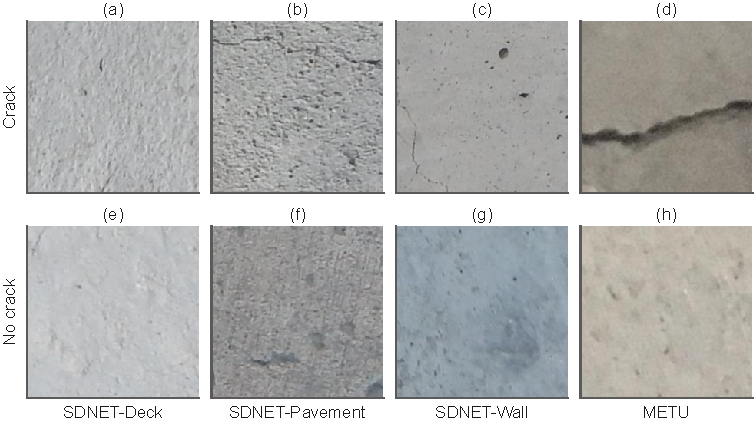
\includegraphics{figures/fig1_muestras_dominios.pdf}
\caption{One cracked (top row) and one uncracked (bottom row) patch of each domain, at the 224$\times$224 input size used for training: SDNET-Deck, SDNET-Pavement, SDNET-Wall and METU from left to right}\label{fig:samples}
\end{figure}

\subsection{Direction of transfer}\label{sec:res-direction}

Table~\ref{tab:direction} groups the 144 off-diagonal cells into the three directional partitions. Cross-surface transfer within SDNET2018 gave F1 0.654, with 48.6\% of its 72 cells above the 0.667 of the always-crack classifier. The two cross-campaign directions fell on opposite sides of it: SDNET2018 to METU gave 0.782 (69.4\% of cells above 0.667) and METU to SDNET2018 gave 0.437 (16.7\%). Over all 144 off-diagonal cells, 66 (45.8\%) exceeded 0.667, one equaled it (F1 exactly 2/3) and 77 fell below it. Falling below that F1 does not make a model uninformative: all 144 cells exceeded the balanced accuracy of the always-crack classifier, 0.5, and the 77 cells below its F1 had balanced accuracy 0.557 to 0.735 and MCC 0.17 to 0.52 (partition means in Table~\ref{tab:anchor}).

\begin{table}[t]
\caption{Crack-class F1 by directional partition (mean $\pm$ SD over cells), percentile bootstrap 95\% CI over training runs (10,000 resamples) and share of cells above 0.667, the F1 of a classifier that labels every patch as cracked}\label{tab:direction}
\begin{tabular*}{\textwidth}{@{\extracolsep\fill}lccccc@{}}
\toprule
Partition & Cells & Runs & F1 & 95\% CI & Cells $>$ 0.667 (\%) \\
\midrule
Within-domain & 48 & 48 & 0.867 $\pm$ 0.082 & 0.845, 0.891 & 100.0 \\
Cross-surface & 72 & 36 & 0.654 $\pm$ 0.092 & 0.631, 0.678 & 48.6 \\
SDNET to METU & 36 & 36 & 0.782 $\pm$ 0.149 & 0.733, 0.830 & 69.4 \\
METU to SDNET & 36 & 12 & 0.437 $\pm$ 0.164 & 0.407, 0.464 & 16.7 \\
\botrule
\end{tabular*}
\end{table}

Figure~\ref{fig:matrix} shows the same pattern cell by cell. The two lowest cells of the mean matrix are in the METU row, METU to SDNET-Wall (0.332) and METU to SDNET-Deck (0.335), and the lowest cell of every architecture panel is one of these two. The highest off-diagonal cell of every panel is in the METU column, SDNET-Pavement to METU, between 0.911 and 0.958 (Tables~\ref{tab:A-cells1} and~\ref{tab:A-cells2}), above the SDNET-Pavement diagonal of the same architecture in all four cases. The METU row averages 0.437 off the diagonal and the METU column 0.782. Within the METU row, METU to SDNET-Pavement (0.645) is the exception. Figure~\ref{fig:bars} shows that in each of the four architectures the two cross-campaign directions lie on either side of the cross-surface partition.

\begin{figure}[t]
\centering
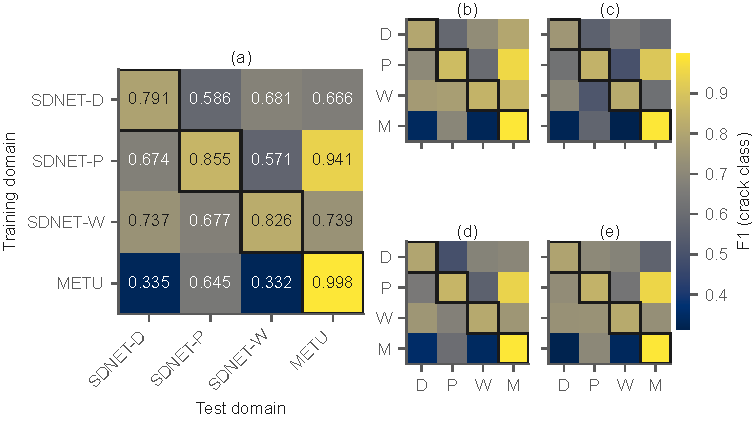
\includegraphics{figures/fig2_matriz_transferencia.pdf}
\caption{Crack-class F1 for every training and test domain, mean over three seeds. (a) Mean over the four architectures; (b) ResNet-18; (c) EfficientNet-B0; (d) MobileNetV3-Small; (e) ViT-Tiny. All panels share one color scale; the boxed diagonal is the within-domain reference. SDNET-D (D), SDNET-P (P) and SDNET-W (W) are the deck, pavement and wall subsets of SDNET2018; M is METU}\label{fig:matrix}
\end{figure}

\begin{figure}[t]
\centering
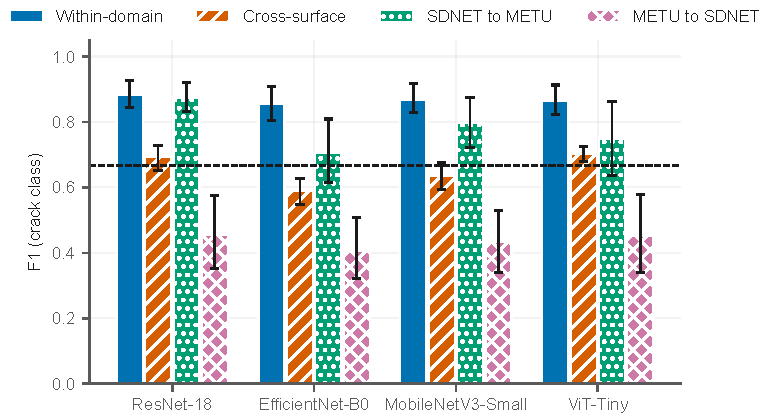
\includegraphics{figures/fig3_f1_por_particion.pdf}
\caption{Crack-class F1 by architecture and directional partition, with percentile bootstrap 95\% confidence intervals over the cells of each bar (10,000 resamples; 9 to 18 cells from 3 to 12 runs). The dashed line at 0.667 is the F1 of a classifier that labels every patch as cracked on these balanced test sets}\label{fig:bars}
\end{figure}

The two-way ANOVA fixed a priori found effects of architecture ($F(3,128)=25.95$, $p<0.0001$, partial eta squared $\eta^2_p=0.38$) and of the train-test pair ($F(15,128)=160.03$, $p<0.0001$, $\eta^2_p=0.95$, a factor that includes the diagonal), and an interaction between them ($F(45,128)=2.79$, $p<0.0001$, $\eta^2_p=0.50$). Its assumptions did not hold: Levene's test rejected equal variances across the three transfer categories (statistic 53.81, $p<0.0001$; variance 0.0067 within domain, 0.0085 cross-surface and 0.0544 cross-campaign) and the Shapiro-Wilk test rejected normal residuals ($W=0.939$, $p<0.0001$). Tukey's HSD on the three a priori categories placed within-domain F1 above cross-surface (difference 0.213, 95\% CI 0.143, 0.283) and above cross-campaign (0.258, CI 0.188, 0.328), and found no difference between cross-surface and cross-campaign (0.045, CI $-0.018$, $+0.107$, $p=0.21$).

The split by direction changes that result (Table~\ref{tab:welch}). With the training run as unit and Holm's correction, five of the six comparisons are significant. Cross-surface transfer is worse than SDNET2018 to METU ($-0.128$, CI $-0.180$, $-0.076$; $r=-0.72$) and better than METU to SDNET2018 ($+0.217$, $\delta=1.00$), and the two cross-campaign directions differ by 0.345 (Welch's $t=11.86$, $\delta=1.00$). The exception is the loss from the SDNET2018 diagonals to METU: paired over the 36 runs with an SDNET2018 source it is 0.042 (CI 0.002, 0.082), not significant after correction ($p_\mathrm{Holm}=0.12$). A Welch test on cells had found this pair significant ($p=0.0031$), but it compared all 48 diagonals, including the METU ones, with cells whose sources are SDNET2018 only. The pooled cross-campaign mean, 0.610, lies between the two directional means and outside the confidence interval of each. Most of the cross-campaign variance that Levene's test flagged comes from pooling the two directions, whose own standard deviations, 0.149 and 0.164, are similar.

\begin{table}[t]
\caption{Pairwise comparison of the directional partitions with the training run as unit: mean difference in F1 (group 1 minus group 2), bootstrap 95\% CI for paired comparisons, Holm-adjusted $p$ over the six comparisons, and effect size (matched-pairs rank-biserial $r$ for paired comparisons, Cliff's $\delta$ for independent ones)}\label{tab:welch}
\setlength{\tabcolsep}{3pt}
\begin{tabular*}{\textwidth}{@{\extracolsep\fill}llccccc@{}}
\toprule
Group 1 & Group 2 & Test & Diff. & 95\% CI & $p$ & Effect \\
\midrule
Within & Cross-surface & SR (36) & $+0.169$ & 0.146, 0.193 & $<$0.0001 & 1.00 \\
Within & SDNET to METU & SR (36) & $+0.042$ & 0.002, 0.082 & 0.12 & 0.30 \\
Within & METU to SDNET & SR (12) & $+0.561$ & 0.534, 0.592 & 0.0010 & 1.00 \\
Cross-surface & SDNET to METU & SR (36) & $-0.128$ & $-0.180$, $-0.076$ & 0.0002 & $-0.72$ \\
Cross-surface & METU to SDNET & $t$ (36/12) & $+0.217$ & 0.182, 0.256 & $<$0.0001 & 1.00 \\
SDNET to METU & METU to SDNET & $t$ (36/12) & $+0.345$ & 0.290, 0.403 & $<$0.0001 & 1.00 \\
\botrule
\end{tabular*}
\footnotetext{SR: Wilcoxon signed-rank test on paired runs (number of runs), effect $r$; $t$: Welch's test on independent runs, effect Cliff's $\delta$. For independent runs the CI resamples runs within each group separately. CIs are not adjusted for multiplicity, so an interval can exclude zero while the Holm-adjusted $p$ exceeds 0.05. In paired comparisons the within-domain value is the diagonal of the same runs: SDNET2018 diagonals (mean 0.824) in the first two rows, METU diagonals (0.998) in the third.}
\end{table}

\subsection{Relative drop by architecture}\label{sec:res-drop}

Table~\ref{tab:drop} gives the relative drop of each off-diagonal cell, anchored on the diagonal of the same model (Equation~\ref{eq:drop}), averaged by architecture and partition. Cross-surface drops ranged from 0.143 (ViT-Tiny) to 0.269 (EfficientNet-B0). SDNET2018-to-METU drops ranged from $-0.037$ for ResNet-18, whose F1 on METU exceeded on average its own SDNET2018 diagonals, to 0.129 for EfficientNet-B0. METU-to-SDNET2018 drops ranged from 0.544 (ResNet-18) to 0.594 (EfficientNet-B0), between two and four times the cross-surface drop of the same architecture.

EfficientNet-B0 had the largest drop in all three partitions. ResNet-18, the largest of the four models, had the smallest drop in both cross-campaign directions, and ViT-Tiny the smallest between surfaces. The ordering follows parameter count in none of the partitions, although from METU to SDNET2018 it comes close to the inverse of it, with MobileNetV3-Small and EfficientNet-B0 swapped. The spread across architectures within a partition was at most 0.165 (SDNET2018 to METU); the spread across partitions for a fixed architecture was at least 0.456 (ViT-Tiny).

Anchoring the drop on the source diagonal favors transfer to METU, whose test set every model scores close to its ceiling. Anchored instead on the within-domain F1 of the target (Table~\ref{tab:anchor}), the drop from SDNET2018 to METU, 0.217, is at least as large as the cross-surface drop, 0.204, while the drop from METU to SDNET2018, 0.474, remains the largest. The ordering of the three partitions by balanced accuracy and by MCC matches their ordering by F1.

\begin{table}[t]
\caption{Measures that do not depend on the source diagonal or favor the always-crack classifier, by directional partition (baseline, mean over cells): relative drop anchored on the source ($\Delta_s$, Equation~\ref{eq:drop}) and on the target ($\Delta_t$) diagonal; balanced accuracy (BA) and MCC at the default threshold and with the threshold chosen by Youden's index on 50 labeled target patches (mean of 200 draws, evaluated on the other 550); and precision at the prevalence of cracked patches in the full target collection}\label{tab:anchor}
\setlength{\tabcolsep}{3pt}
\begin{tabular*}{\textwidth}{@{\extracolsep\fill}lccccccc@{}}
\toprule
 & & & \multicolumn{2}{c}{Threshold 0.5} & \multicolumn{2}{c}{Youden, $k=50$} & Precision at \\
Partition & $\Delta_s$ & $\Delta_t$ & BA & MCC & BA & MCC & prevalence \\
\midrule
Within-domain & -- & -- & 0.871 & 0.744 & 0.863 & 0.733 & 0.628 \\
Cross-surface & 0.205 & 0.204 & 0.709 & 0.448 & 0.712 & 0.446 & 0.454 \\
SDNET to METU & 0.055 & 0.217 & 0.812 & 0.638 & 0.810 & 0.635 & 0.870 \\
METU to SDNET & 0.562 & 0.474 & 0.629 & 0.332 & 0.656 & 0.349 & 0.538 \\
\botrule
\end{tabular*}
\footnotetext{The always-crack classifier scores BA 0.5 and MCC 0. Prevalence: 14.9\%, 10.7\% and 21.2\% for SDNET-Deck, -Pavement and -Wall, 50\% for METU. These analyses are described in Section~\ref{sec:stats} and were added after the results were known.}
% Origen: results/tables/ronda2_particiones.csv y ronda2.json (src/09_ronda2.py).
\end{table}

\begin{table}[t]
\caption{Relative F1 drop per off-diagonal cell (mean $\pm$ SD over cells), anchored on the within-domain F1 of the same architecture, seed and source domain. Smallest drop per column in bold; a negative drop is a gain over the source diagonal}\label{tab:drop}
\begin{tabular*}{\textwidth}{@{\extracolsep\fill}lccc@{}}
\toprule
Architecture & Cross-surface & SDNET to METU & METU to SDNET \\
\midrule
ResNet-18 & 0.179 $\pm$ 0.104 & \textbf{$-$0.037 $\pm$ 0.055} & \textbf{0.544 $\pm$ 0.183} \\
EfficientNet-B0 & 0.269 $\pm$ 0.119 & 0.129 $\pm$ 0.163 & 0.594 $\pm$ 0.152 \\
MobileNetV3-Small & 0.230 $\pm$ 0.116 & 0.036 $\pm$ 0.120 & 0.565 $\pm$ 0.154 \\
ViT-Tiny & \textbf{0.143 $\pm$ 0.062} & 0.090 $\pm$ 0.202 & 0.546 $\pm$ 0.190 \\
\botrule
\end{tabular*}
\end{table}

\subsection{Precision and recall}\label{sec:res-pr}

Out of domain the models lost much more recall than precision (Table~\ref{tab:pr}). Mean precision stayed between 0.807 and 0.870 in the three off-diagonal partitions, against 0.886 within domain, while recall fell from 0.851 within domain to 0.728 from SDNET2018 to METU, 0.577 between surfaces and 0.320 from METU to SDNET2018. Missed cracks made up 57.9\% of the errors within domain and 91.7\% of the errors from METU to SDNET2018. Per training run, precision exceeded recall in every off-diagonal partition, in all 12 runs from METU to SDNET2018 (mean difference 0.538, CI 0.497, 0.582). Of the 78 off-diagonal cells at or below the always-crack F1 (77 below, one tie), 77 had precision above recall, with mean precision 0.838 and mean recall 0.384. No cell lacked positive predictions; the fewest positive predictions in a cell was 40 of 600.

These precisions hold on balanced test sets. At the prevalence of cracked patches in the full SDNET2018 subsets, the same true- and false-positive rates give a mean precision of 0.538 from METU to SDNET2018 (0.364 on SDNET-Pavement, 0.477 on SDNET-Deck and 0.773 on SDNET-Wall) and 0.454 between surfaces (Table~\ref{tab:anchor}): at those prevalences, about half of the cracks such a model reports would be false alarms. The prevalence of an inspection in the field depends on the structure and on how its images are cut into patches, and was not measured.

\begin{table}[t]
\caption{Precision and recall of the crack class by directional partition (mean $\pm$ SD over cells), share of missed cracks (false negatives, FN) among all errors, and paired difference between precision and recall (P $-$ R) per training run (Wilcoxon signed-rank test, Holm's correction over three partitions, matched-pairs rank-biserial correlation $r$)}\label{tab:pr}
\begin{tabular*}{\textwidth}{@{\extracolsep\fill}lcccccc@{}}
\toprule
Partition & Precision & Recall & FN share (\%) & P $-$ R & $p$ (Holm) & $r$ \\
\midrule
Within-domain & 0.886 $\pm$ 0.073 & 0.851 $\pm$ 0.094 & 57.9 & -- & -- & -- \\
Cross-surface & 0.807 $\pm$ 0.085 & 0.577 $\pm$ 0.154 & 72.7 & $+0.230$ & $<$0.0001 & 0.86 \\
SDNET to METU & 0.870 $\pm$ 0.092 & 0.728 $\pm$ 0.196 & 72.4 & $+0.142$ & $<$0.0001 & 0.82 \\
METU to SDNET & 0.857 $\pm$ 0.069 & 0.320 $\pm$ 0.178 & 91.7 & $+0.538$ & 0.0005 & 1.00 \\
\botrule
\end{tabular*}
\footnotetext{Runs per partition: 36, 36 and 12. 95\% bootstrap CI of P $-$ R: $+0.164$, $+0.290$; $+0.092$, $+0.195$; $+0.497$, $+0.582$.}
\end{table}

Figure~\ref{fig:pr} places every cell in the precision-recall plane. The always-crack classifier sits at recall 1.0 and precision 0.5; the cells that fall below its F1 lie at the opposite corner, with high precision and low recall. From METU to SDNET-Deck and SDNET-Wall, recall did not exceed 0.317 in any of the 24 cells, with mean precision 0.828 and 0.920.

\begin{figure}[t]
\centering
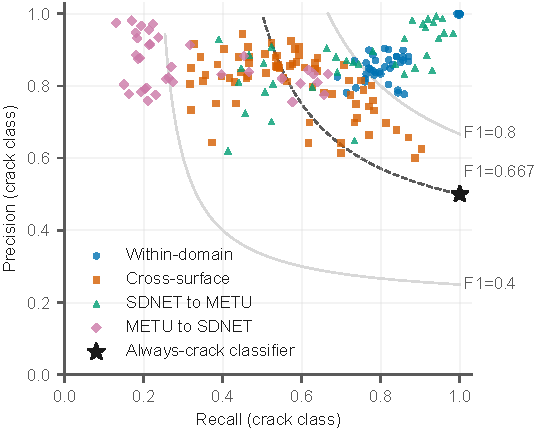
\includegraphics{figures/fig5_precision_recall.pdf}
\caption{Precision against recall of the crack class for the 192 cells of the baseline condition. Gray curves are iso-F1 lines, the dashed one at 0.667; the star is the classifier that labels every patch as cracked}\label{fig:pr}
\end{figure}

Figure~\ref{fig:errors} shows errors of one model from the pair with the lowest mean F1, EfficientNet-B0 trained on METU and tested on SDNET-Wall (mean over seeds 0.313). The model is the seed with the median F1 of the three (seed 43, F1 0.299), one of the 48 baseline runs. On the 300 cracked and 300 uncracked test patches it produced 54 true positives, 246 false negatives, 7 false positives and 293 true negatives: precision 0.89, recall 0.18. Panels (a) to (c) are the three false positives with the highest predicted crack probability: a straight dark line across the patch, the broken edge of a large hole and a small cavity. Panels (d) to (f) are the three false negatives with the lowest probability, all thin cracks of low contrast against the surface texture. These are the extremes of one model, selected by a fixed rule, and not a quantified classification of errors; some of them may be ambiguous labels rather than model errors, since the labels were not audited.

\subsection{Ranking and decision threshold}\label{sec:res-threshold}

A loss of recall at a fixed threshold of 0.5 can mean that the model does not separate the classes of the target domain, or that it separates them but the threshold learned on the source no longer fits. Table~\ref{tab:threshold} separates the two. From METU to SDNET2018 the models ranked target patches much worse than within domain: mean AUROC 0.699 against 0.927, 0.679 on SDNET-Deck and 0.627 on SDNET-Wall, with 20 of the 36 cells below 0.70. Choosing the threshold on 50 labeled target patches to maximize F1 raised mean F1 from 0.437 to 0.673, and the best threshold on the whole test set to 0.696. The second figure cannot fall below 0.667, because the lowest threshold labels every patch as cracked, and the first is pulled toward that value, because maximizing F1 favors low thresholds: for an uninformative classifier it labels every example as positive, and a threshold chosen on a small sample overfits it \citep{lipton2014}. From METU to SDNET2018 the F1-chosen threshold lowered MCC from 0.332 to 0.205. A threshold chosen on the same 50 patches by Youden's index raised balanced accuracy only from 0.629 to 0.656 and MCC from 0.332 to 0.349 (Table~\ref{tab:anchor}); between surfaces and from SDNET2018 to METU it changed neither by more than 0.004. The default threshold therefore accounts for little of the loss, and the ranking of target patches for more. Within domain a threshold chosen on 50 patches scored slightly below the default one, which was already fitted to that domain. The linear probe ranked METU-to-SDNET2018 patches slightly better than fine-tuning (AUROC 0.735).

\begin{table}[t]
\caption{Ranking and threshold by directional partition (fine-tuning, mean over cells): AUROC, AP, F1 at the default threshold of 0.5, F1 with the threshold chosen to maximize F1 on $k$ labeled target patches and evaluated on the other $600-k$ (mean of 200 draws), and F1 at the best threshold on the whole test set. The last four columns cannot fall far below 0.667, the F1 of labeling every patch as cracked, which is among the thresholds considered; Table~\ref{tab:anchor} gives a threshold criterion that does not favor it}\label{tab:threshold}
\begin{tabular*}{\textwidth}{@{\extracolsep\fill}lccccccc@{}}
\toprule
Partition & AUROC & AP & F1 (0.5) & $k=20$ & $k=50$ & $k=100$ & Best \\
\midrule
Within-domain & 0.927 & 0.940 & 0.867 & 0.840 & 0.854 & 0.860 & 0.875 \\
Cross-surface & 0.782 & 0.817 & 0.654 & 0.692 & 0.705 & 0.711 & 0.731 \\
SDNET to METU & 0.847 & 0.868 & 0.782 & 0.782 & 0.799 & 0.806 & 0.822 \\
METU to SDNET & 0.699 & 0.707 & 0.437 & 0.651 & 0.673 & 0.682 & 0.696 \\
\botrule
\end{tabular*}
\end{table}

\begin{figure}[t]
\centering
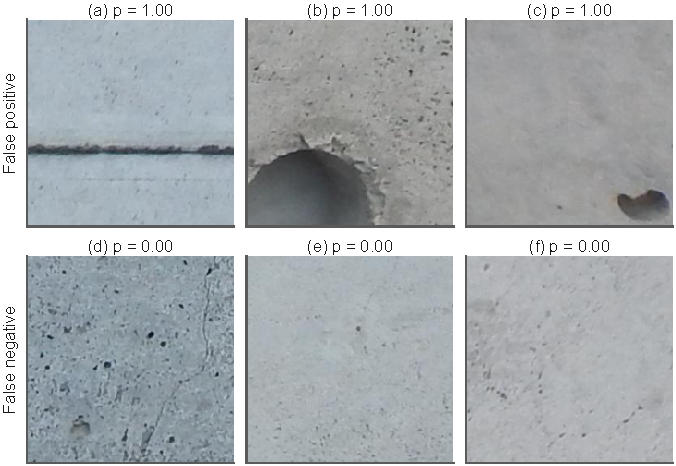
\includegraphics{figures/fig4_errores.pdf}
\caption{Errors of EfficientNet-B0 trained on METU and tested on SDNET-Wall (seed 43, F1 0.299; 54 TP, 246 FN, 7 FP, 293 TN). (a--c) The three false positives with the highest predicted crack probability $p$; (d--f) the three false negatives with the lowest. Probabilities rounded to two decimals}\label{fig:errors}
\end{figure}

\subsection{Training-time interventions}\label{sec:res-interventions}

Neither aggressive augmentation nor histogram equalization improved out-of-domain F1. Per training run, averaging its three off-diagonal cells, aggressive augmentation changed F1 by $-0.005$ (95\% CI $-0.028$, $+0.019$; Wilcoxon $p=0.76$, $r=-0.05$) and histogram equalization by $-0.027$ (CI $-0.051$, $-0.004$; $p=0.048$, $p_\mathrm{Holm}=0.095$, $r=-0.33$), a small loss whose interval excludes zero but which does not survive the correction for two comparisons. Both interventions lowered within-domain F1, from 0.867 to 0.834 with augmentation and 0.823 with equalization. Augmentation lowered it mostly on SDNET-Deck (0.791 to 0.728) and SDNET-Wall (0.826 to 0.771); equalization lowered it on all three SDNET2018 subsets (to 0.722, 0.806 and 0.769 on SDNET-Deck, -Pavement and -Wall). The share of off-diagonal cells above 0.667 was 51.4\% with augmentation and 42.4\% with equalization, against 45.8\% for the baseline.

Scale augmentation did not meet its primary test (Table~\ref{tab:scale}). From METU to SDNET2018, mean F1 per run rose from 0.437 to 0.492 (difference $+0.055$, CI $+0.010$, $+0.098$; Wilcoxon $W=14$, $p=0.052$, $r=0.64$), and 9 of the 12 runs improved. The mean change by architecture was $+0.054$ for EfficientNet-B0, $+0.102$ for MobileNetV3-Small, $+0.064$ for ViT-Tiny and $-0.001$ for ResNet-18. The gain came from recall (0.320 to 0.379, precision 0.857 to 0.842), not from ranking: AUROC moved from 0.699 to 0.706, and with the threshold chosen on 50 labeled target patches F1 was 0.675 against 0.673 for the baseline. No secondary comparison was significant after correction. The bootstrap interval of the primary difference excludes zero while the test does not reach $\alpha=0.05$; with 12 runs the result is inconclusive rather than negative. Unlike the other two interventions, scale augmentation did not lower within-domain F1 (0.870 against 0.867). Over all 144 off-diagonal cells, 50.0\% exceeded 0.667, and 71 of the 72 cells at or below it kept precision above recall.

\begin{table}[t]
\caption{Scale augmentation against the baseline, per training run: mean of each run's cells in the partition, paired difference (scale minus baseline) with 95\% bootstrap CI, Wilcoxon signed-rank test and rank-biserial correlation $r$. The primary test was fixed before training; Holm's correction applies to the five secondary comparisons}\label{tab:scale}
\setlength{\tabcolsep}{3pt}
\begin{tabular*}{\textwidth}{@{\extracolsep\fill}llcccccc@{}}
\toprule
Comparison & Runs & Baseline & Scale & Diff. & 95\% CI & $p$ & $r$ \\
\midrule
\multicolumn{8}{@{}l}{\textit{Primary}} \\
F1, METU to SDNET & 12 & 0.437 & 0.492 & $+0.055$ & $+0.010$, $+0.098$ & 0.052 & 0.64 \\
\multicolumn{8}{@{}l}{\textit{Secondary} ($p$ with Holm's correction)} \\
Recall, METU to SDNET & 12 & 0.320 & 0.379 & $+0.060$ & $+0.013$, $+0.106$ & 0.21 & 0.67 \\
AUROC, METU to SDNET & 12 & 0.699 & 0.706 & $+0.006$ & $-0.013$, $+0.026$ & 0.86 & 0.13 \\
F1, cross-surface & 36 & 0.654 & 0.663 & $+0.008$ & $-0.010$, $+0.027$ & 0.86 & 0.20 \\
F1, SDNET to METU & 36 & 0.782 & 0.760 & $-0.022$ & $-0.058$, $+0.010$ & 0.86 & $-0.21$ \\
F1, within-domain & 48 & 0.867 & 0.870 & $+0.003$ & $-0.003$, $+0.008$ & 0.25 & 0.33 \\
\botrule
\end{tabular*}
% Origen: results/tables/exp_escala.json (04_stats.py, funcion exp_escala).
\end{table}

\subsection{Linear probe against fine-tuning}\label{sec:res-probe}

A linear classifier on frozen ImageNet features reached a within-domain F1 of 0.851, against 0.867 for fine-tuning, and 0.997 on METU. Relative to its own diagonal it lost less than fine-tuning in the two partitions with an SDNET2018 source and no differently in the third (Table~\ref{tab:probe}, Figure~\ref{fig:probe}). Between surfaces the drop was 0.154 against 0.205 (paired difference 0.051, CI 0.031, 0.070, Holm $p<0.0001$); from SDNET2018 to METU the probe gained slightly ($-0.030$) where fine-tuning lost 0.055. From METU to SDNET2018 the two regimes did not differ (0.597 against 0.562, $p=0.15$). In absolute F1 the differences were smaller: the probe scored 0.023 and 0.046 above fine-tuning in the two SDNET2018-source partitions and 0.035 below it from METU to SDNET2018. From METU to SDNET2018 the probe failed in the same way as the fine-tuned models, with recall 0.305 and precision 0.825. Overall, 54.9\% of the probe's off-diagonal cells exceeded 0.667.

\begin{table}[t]
\caption{Linear probe on frozen features (LP) against fine-tuning (FT), per training run and partition: mean out-of-domain F1, mean relative drop $\Delta$ (Equation~\ref{eq:drop}), paired difference of the drops (Diff., FT minus LP) with 95\% bootstrap CI, Wilcoxon signed-rank test with Holm's correction and rank-biserial correlation $r$. Within-domain F1: FT 0.867, LP 0.851}\label{tab:probe}
\begin{tabular*}{\textwidth}{@{\extracolsep\fill}lcccccccc@{}}
\toprule
Partition & Runs & F1 FT & F1 LP & $\Delta$ FT & $\Delta$ LP & Diff. & $p$ & $r$ \\
\midrule
Cross-surface & 36 & 0.654 & 0.678 & 0.205 & 0.154 & $+0.051$ & $<$0.0001 & 0.81 \\
SDNET to METU & 36 & 0.782 & 0.828 & 0.055 & $-0.030$ & $+0.085$ & 0.0003 & 0.70 \\
METU to SDNET & 12 & 0.437 & 0.402 & 0.562 & 0.597 & $-0.034$ & 0.15 & $-0.49$ \\
\botrule
\end{tabular*}
\footnotetext{95\% bootstrap CI of the difference: $+0.031$, $+0.070$; $+0.046$, $+0.125$; $-0.073$, $+0.003$.}
\end{table}

\begin{figure}[t]
\centering
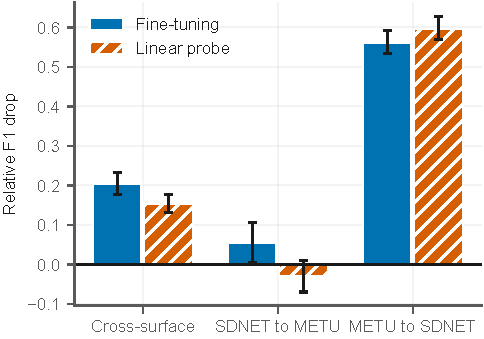
\includegraphics{figures/fig6_sonda_frente_ajuste.pdf}
\caption{Mean relative F1 drop of fine-tuning and of the linear probe by directional partition, with percentile bootstrap 95\% confidence intervals over training runs}\label{fig:probe}
\end{figure}

\subsection{Three sources, one domain held out}\label{sec:res-multisource}

Trained on three domains with the data budget of one, the models scored above the mean of the three single-source models on every held-out domain (Table~\ref{tab:multi}, Figure~\ref{fig:multi}). Over the 48 paired runs the difference was $+0.134$ (CI $+0.116$, $+0.152$; Holm $p<0.0001$; $r=1.00$). Against the best of the three single-source models, chosen after the fact on the held-out test set, the difference was $-0.004$ (CI $-0.017$, $+0.009$; $p=0.42$; $r=-0.14$). The test does not establish equivalence. On the three SDNET2018 subsets the three-source model scored slightly above that best single source; with METU held out it scored 0.903, below the 0.941 of the model trained on SDNET-Pavement alone. The composition of the sources differs between these cases: with an SDNET2018 subset held out, two of the three sources come from the same collection as the target, and with METU held out all three come from SDNET2018. On the test sets of their own source domains the three-source models scored 0.776, 0.835, 0.789 and 0.995 for SDNET-Deck, -Pavement, -Wall and METU, close to the single-source diagonals although each source supplied a third of the training data.

\begin{table}[t]
\caption{F1 on the held-out domain of the three-source model and of the single-source models of the same architecture and seed (mean $\pm$ SD over 4 architectures $\times$ 3 seeds), and recall of the three-source model}\label{tab:multi}
\begin{tabular*}{\textwidth}{@{\extracolsep\fill}lcccc@{}}
\toprule
Held-out domain & Three sources & One source, mean & One source, best$^\dagger$ & Recall (three) \\
\midrule
SDNET-Deck & 0.742 $\pm$ 0.025 & 0.582 $\pm$ 0.036 & 0.740 $\pm$ 0.034 & 0.736 $\pm$ 0.054 \\
SDNET-Pavement & 0.723 $\pm$ 0.070 & 0.636 $\pm$ 0.075 & 0.717 $\pm$ 0.052 & 0.674 $\pm$ 0.112 \\
SDNET-Wall & 0.696 $\pm$ 0.044 & 0.528 $\pm$ 0.041 & 0.684 $\pm$ 0.042 & 0.589 $\pm$ 0.057 \\
METU & 0.903 $\pm$ 0.045 & 0.782 $\pm$ 0.077 & 0.941 $\pm$ 0.024 & 0.980 $\pm$ 0.026 \\
\botrule
\end{tabular*}
\footnotetext{$^\dagger$Oracle: the best of the three single sources is chosen on the held-out test set, which an operator cannot do without labeled images of the target.}
\end{table}

\begin{figure}[t]
\centering
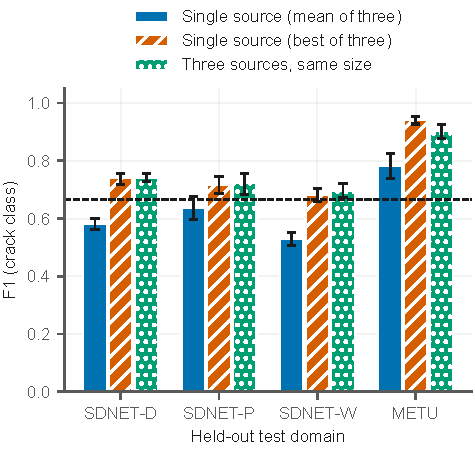
\includegraphics{figures/fig7_multifuente.pdf}
\caption{F1 on each held-out domain of the single-source models (mean of the three sources, and best of the three chosen on the held-out test set) and of the three-source model trained on the same number of patches. Bars: mean over architectures and seeds; whiskers: percentile bootstrap 95\% confidence intervals. Dashed line: F1 of the always-crack classifier}\label{fig:multi}
\end{figure}

\subsection{Sensitivity to the split}\label{sec:res-sensitivity}

Grouping the SDNET2018 splits by parent photograph left the within-domain F1 of SDNET-Deck and SDNET-Wall unchanged within their confidence intervals and lowered that of SDNET-Pavement by 0.024 (Table~\ref{tab:sens}). METU kept its split, and its models and diagonal were identical under both splits. The directional means under the grouped split were 0.860 within domain, 0.681 between surfaces, 0.757 from SDNET2018 to METU and 0.492 from METU to SDNET2018; 54.9\% of off-diagonal cells exceeded 0.667. The METU-to-SDNET2018 cells changed because the SDNET2018 test sets are different patches under the grouped split, not because the METU models changed: replacing the test patches alone moved that partition by 0.055. The two cross-campaign directions still differed by 0.265 with the training run as unit (Welch's $t=8.02$, $p<0.0001$), against 0.345 under the patch-level split, and the relative drops were 0.164 between surfaces, 0.072 from SDNET2018 to METU and 0.507 from METU to SDNET2018, against 0.205, 0.055 and 0.562.

\begin{table}[t]
\caption{Within-domain F1 under the patch-level split and the split grouped by parent photograph (baseline condition, mean over 4 architectures $\times$ 3 seeds), paired difference and percentile bootstrap 95\% CI}\label{tab:sens}
\begin{tabular*}{\textwidth}{@{\extracolsep\fill}lcccc@{}}
\toprule
Domain & Patch split & Photo-grouped split & Difference & 95\% CI \\
\midrule
SDNET-Deck & 0.791 & 0.787 & $-0.004$ & $-0.022$, $+0.014$ \\
SDNET-Pavement & 0.855 & 0.831 & $-0.024$ & $-0.034$, $-0.011$ \\
SDNET-Wall & 0.826 & 0.823 & $-0.003$ & $-0.015$, $+0.010$ \\
METU & 0.998 & 0.998 & 0.000 & n/a \\
\botrule
\end{tabular*}
\footnotetext{METU keeps its split (file names carry no photograph identifier), so its models are identical under both splits. The grouped split has 1,390 training patches per class in each SDNET2018 subset instead of 1,400.}
\end{table}

% =====================================================================
\section{Discussion}\label{sec:discussion}

\subsection{Within-domain performance by domain}\label{sec:disc-diagonal}

The a priori hypothesis (Section~\ref{sec:matrix}) had four parts. Within-domain F1 reached the assumed 0.97 in one domain of four. F1 fell on leaving the training domain on average in every partition, but not in every cell, and the loss from the SDNET2018 diagonals to METU was small and not significant after correction. The predicted ordering of the partitions and the predicted effect of model size did not hold.

Every architecture separates METU at 0.998 or above, and so does a linear classifier on frozen ImageNet features (0.997), so the METU decision is close to linearly separable in generic pretrained features. The SDNET2018 subsets stay between 0.754 and 0.874 for every architecture. Subsampling to 2,000 patches per class and training for at most 12 epochs apply to all four domains alike; they may interact with the difficulty or the label noise of a domain, but they do not by themselves create a gap of 0.21 between domains. Leakage between patches of the same photograph does not explain it either: it can only inflate the SDNET2018 diagonals, and removing it lowered them by at most 0.024 (Section~\ref{sec:res-sensitivity}).

One candidate explanation is how the patches were framed. The cracked METU patches are close-ups with the crack centered in the patch, labeled as cracked only when the crack lies at least 5 pixels from the patch edges \citep{santos2022}. SDNET2018 patches were cut on a regular grid from photographs of a surface, and the collection includes cracks as narrow as 0.06~mm \citep{dorafshan2018sdnet}, so a crack can be thin or lie near the edge of a patch. \citet{fountoukidou2024} traced part of their synthetic-to-real gap to a similar difference, close-ups against overall views. This study did not measure crack width or position in the patch. It tested the explanation indirectly, by training with random rescaling, and the result did not meet the criterion fixed for it (Section~\ref{sec:disc-regime}).

\subsection{Direction of transfer and architecture}\label{sec:disc-direction}

The predicted ordering did not hold because the two cross-campaign directions differed. Measured from the diagonals of the source runs, training on SDNET2018 and testing on METU cost less than moving between two SDNET2018 surfaces, and training on METU and testing on SDNET2018 cost more than three times the cross-surface loss (0.561 against 0.169). Measured as a relative drop from the diagonal of the target ($\Delta_t$, Table~\ref{tab:anchor}), the first comparison does not hold: SDNET2018-to-METU transfer drops by 0.217 and cross-surface transfer by 0.204, while METU-to-SDNET2018 transfer still drops most (0.474). In absolute F1 below the target diagonal the first comparison reverses (0.216 against 0.169). Part of the asymmetry in absolute F1 therefore reflects that METU is an easy target, on which every model starts close to its ceiling; the part that holds under either anchor is the large loss of METU-trained models on SDNET2018. The analysis fixed before the first runs pooled the two directions and found cross-campaign transfer no worse than cross-surface transfer, a conclusion that each direction, taken alone, contradicts; the pooled mean of 0.610 lies outside the confidence interval of both. A cross-dataset evaluation therefore needs both directions of each pair, as in the matrix of \citet{torralba2011}. The cross-testing matrix of \citet{rashid2025} contains both directions with one run per configuration, but its SDNET2018 test set kept the imbalance of the collection, so accuracy rewarded models that label few patches as cracked. There, models trained on the METU collection scored 76--84\% accuracy on SDNET2018, at or above the reverse direction for all four models, while F1 favored the reverse direction for two of them. Here the test sets are balanced and each comparison uses replicated runs; the asymmetry holds for all four architectures and under the photo-grouped split (0.265). \citet{santos2022} observed the same direction with a different target: a classifier trained on METU fell to 54\% accuracy on patches of a concrete dam.

The cross-surface control is not a pure change of surface: the SDNET2018 decks were photographed in a laboratory and the walls and pavements on campus (Section~\ref{sec:data}), so pairs involving the decks also change site. The two pairs that keep the site, walls and pavements in both directions, average 0.624, against 0.669 for the four pairs with the decks; this difference was not tested, but the pairs that change site did not transfer worse in this collection.

The asymmetry admits two explanations. One is relative difficulty: a model fitted to a domain where the decision is nearly separable may not learn features that survive a harder domain, while a model fitted to a harder domain may carry features that also work on an easier one. The other is a shortcut in the sense of \citet{geirhos2020}: a decision rule fitted to the centered close-ups of METU would solve the in-domain test and miss the thinner, off-center cracks of SDNET2018 patches. Three results are relevant to both. The failure is a loss of recall at high precision on the balanced test sets (Section~\ref{sec:res-pr}): METU-trained models label most SDNET2018 cracks as uncracked. The threshold accounts for little of it: the same models rank SDNET-Deck and SDNET-Wall patches much worse than within domain (AUROC 0.68 and 0.63), and a threshold chosen by Youden's index on 50 target patches raises balanced accuracy only from 0.629 to 0.656 (Section~\ref{sec:res-threshold}). The linear probe trained on METU also fails in the same way (recall 0.305, AUROC 0.735), so for these ImageNet-pretrained models the loss does not come from fine-tuning distorting the features. The features themselves can separate SDNET2018 cracks, since probes trained on SDNET2018 reach 0.781 to 0.830 on their own subsets (Table~\ref{tab:A-regimes}); what does not transfer is the boundary learned on METU. Both explanations predict the observed direction. Only the first predicts that the within-domain F1 of a source forecasts how well it transfers, which would be useful because the diagonal can be measured before any target data exist. Across models evaluated under one distribution shift, out-of-distribution accuracy is often strongly correlated with in-distribution accuracy \citep{miller2021}; the hypothesis here concerns sources rather than models, and with two collections it cannot be tested. For this pair of collections transfer differed by direction, so a single number per dataset pair, which assumes a symmetric distance between them, would have misdescribed it.

The hypothesis that larger architectures lose more did not hold. ResNet-18, the largest model tested, had the smallest drop in both cross-campaign directions, and EfficientNet-B0, in the middle by parameter count, had the largest in every partition. The spread across architectures within a partition (at most 0.165) is small next to the spread across partitions for a fixed architecture (at least 0.456), and the architecture $\times$ pair interaction ($\eta^2_p=0.50$) indicates that which architecture transfers best depends on the pair. \citet{ozgenel2018} found a stronger architecture effect for networks trained on METU: the best accuracy of VGG16 on three external test sets was 0.96 to 0.98, against 0.54 to 0.77 for ResNet101 and ResNet152. Their figures are maxima over training-set sizes and epochs on each test set, and their networks reach 144 million parameters, so the two studies cover different conditions; here no size effect was detected between 1.52 and 11.18 million parameters, with four models.

\subsection{What the training regime changes}\label{sec:disc-regime}

Aggressive augmentation and histogram equalization did not reduce the loss, and both cost within-domain F1 on the SDNET2018 subsets. Both act on orientation and on photometric properties such as contrast, not on scale, the property that the framing explanation points to.

Scale augmentation was added to test that explanation, with a primary test fixed before training and a reading fixed with it: a significant gain from METU to SDNET2018 would support the explanation without proving it, and its absence would weaken it. The gain was $+0.055$ F1 with $p=0.052$, and its bootstrap interval excluded zero. The test was not met, so by the reading fixed in advance the explanation is weakened; with 12 runs the result is inconclusive rather than a refutation. Two other results are consistent with a weak role for scale. The gain came from recall at a fixed threshold, while AUROC did not change and a threshold recalibrated on 50 target patches gave the same F1 with and without the augmentation; rescaling moved the operating point of METU-trained models but did not make them separate SDNET2018 cracks better. Even if real, the gain would close about one seventh of the gap of 0.387 between the METU-to-SDNET2018 cells and the mean SDNET2018 diagonal (0.824). Training on rescaled METU patches does not reproduce what distinguishes SDNET2018 cracks; whether a difference in crack width, which rescaling changes together with everything else in the patch, or other properties of the collections account for the loss remains open.

The linear probe tests the account of \citet{kumar2022}, in which fine-tuning distorts good pretrained features and loses out of distribution against a linear probe when the shift is large. The probe lost less than fine-tuning relative to its own diagonal when the source was SDNET2018, but not under the largest shift, from METU to SDNET2018, and in absolute F1 the two regimes differed by less than 0.05 in every partition. Part of the smaller relative drop comes from the probe's lower diagonal. For these models, feature distortion accounts at most for part of the loss between SDNET2018 surfaces and for none of the asymmetry between campaigns; larger pretrained models were not tested.

At the same data budget, the three-source model beat the average single source by 0.134 F1 and did not differ detectably from the best single source, in line with the finding of \citet{gulrajani2021} that standard training on pooled source domains is hard to beat for domain generalization. The best single source can be identified only by testing on the held-out domain; an operator deploying to a new site can do so only with labeled images of that site, the sample that the local validation step of Section~\ref{sec:disc-implications} requires. When METU was held out, all three sources came from SDNET2018 and one of them, SDNET-Pavement, transferred better alone (0.941 against 0.903), so the design measures the pooling of surfaces and sites more than the pooling of campaigns. Methods that use target-domain data during training address the gap differently \citep{wang2018}: adversarial adaptation with unlabeled dam patches raised a METU-trained classifier from 54\% to 84\% accuracy \citep{santos2022}, pseudo-label adaptation between SDNET2018 subsets reached above 95\% accuracy \citep{zhu2026concracknet}, and adaptation of a crack segmentation model needed as few as 100 images of the new site \citep{chun2024}. They were outside the scope of this design.

\subsection{Implications for automated infrastructure inspection}\label{sec:disc-implications}

For an agency deciding whether to deploy a crack classifier trained on a public dataset, the main result is the mode of failure. More than half of the out-of-domain cells here (77 below and one at the F1 of a classifier that reports a crack in every patch) fell to that level, although all of them remained better than chance in balanced accuracy, and 77 of those 78 kept precision above recall. Such a model misses most cracks. On a balanced test set most of the cracks it reports are real; at the prevalence of the SDNET2018 subsets about half of them would be false alarms (Section~\ref{sec:res-pr}). Its missed cracks can be found only with labeled images that include cracks, not by reviewing the patches it flags.

We suggest four steps before such a model informs maintenance decisions. First, collect a labeled sample from the structures to be inspected, including cracked patches, spread over many photographs and structures. With 300 independent cracked patches the 95\% interval of a recall estimate is no wider than $\pm0.06$ under the normal approximation; patches of one photograph are correlated, so a sample concentrated in a few photographs gives a wider interval. Second, measure precision and recall separately on that sample, because F1 or accuracy alone does not show whether the model over-reports or misses cracks, and missed cracks are the error that checking flagged patches cannot reveal. The same sample can be used to choose the decision threshold, by a criterion such as Youden's index rather than by maximizing F1, which drifts toward labeling every patch as cracked \citep{lipton2014}. Here a new threshold changed balanced accuracy little in every partition (Section~\ref{sec:res-threshold}), so a model that ranks the patches of the site poorly is unlikely to be repaired by it; adaptation with images of the site \citep{santos2022, chun2024} is the alternative to evaluate. Third, if labeled images from more than one earlier site are available, train on them pooled; choosing a single source requires testing each on the site sample. Fourth, when publishing an evaluation, report both directions of each dataset pair, a threshold-free measure such as AUROC, a measure that gives the trivial classifier no credit, such as balanced accuracy or MCC, and the F1 of the trivial classifier on the same test set. The first two steps follow from the requirement that a test set represent the conditions of use and be independent of the training data, and are the kind of check on prediction validity after deployment that \citet{hasan2025} recommend. Neither of them requires retraining the model.

% =====================================================================
\section{Limitations}\label{sec:limitations}

First, only two independent capture campaigns are compared, and the asymmetry between them rests on a single pair of collections: a change of campaign here is a change to or from METU, and cannot be separated from the properties of that collection, including how it defines and frames a cracked patch. The explanations offered in Section~\ref{sec:disc-direction} are post hoc. Separating them requires a third campaign whose within-domain F1 falls between the two measured here.

Second, the explanation by framing rests on descriptions of the collections, not on measurements: crack width and position in the patch were not measured, and the labels were not audited. The one direct test, scale augmentation, was added after the other results, used a single range of factors (0.5 to 1.5) fixed before training, and with 12 runs had limited power to detect a gain of the size observed; a wider range or augmentation of crack width alone could give a different answer. SDNET2018 includes cracks as narrow as 0.06~mm, and some patches may be ambiguous, which would lower its diagonals and the METU-to-SDNET2018 cells alike.

Third, subsampling to 2,000 patches per class and at most 12 epochs with early stopping kept within-domain F1 on the SDNET2018 subsets between 0.754 and 0.874, while \citet{dorafshan2018sdnet} reported 87.5--95.5\% accuracy within each subset with all of its data, a different metric on a different split. The matrix therefore describes what these diagonals predict about a new site, and the relative drops, anchored on them, could change with a larger training budget. The subsample, the split and the three-source sample were each drawn once with a fixed seed, so the intervals reported cover variation between training runs at a fixed partition, not variation across draws of the data. Replacing only the SDNET2018 test patches moved the METU-to-SDNET2018 mean by 0.055 (Section~\ref{sec:res-sensitivity}); differences of that size or smaller, such as those between the linear probe and fine-tuning in absolute F1, between the interventions and the baseline, and between pooled and best single sources, are specific to this draw. All test sets were balanced, so precision and F1 describe a prevalence of 50\%; at a lower prevalence, such as that of the full SDNET2018 subsets, the precision of every model would be lower. The prevalence of a real inspection was not measured, and the analyses of Table~\ref{tab:anchor} that address this were added after the results were known.

Fourth, no hyperparameter search was run per architecture, and parameter count varies together with design family and pretraining across the four models: ViT-Tiny was pretrained on ImageNet-21k before ImageNet-1k, and each set of weights comes from a different training recipe (Table~\ref{tab:arch}). The absence of a size effect holds for this range and these models only. All models were small and pretrained on ImageNet: the conclusion of the linear probe does not extend to larger pretrained models, and the combination of probing followed by fine-tuning proposed by \citet{kumar2022} was not tested.

Fifth, the photo-grouped split was run for the baseline condition only, and METU could not be grouped because its file names do not identify the photograph. The METU diagonal may therefore include some leakage between patches of the same photograph; this would affect the relative drops anchored on it, not the absolute F1 of the METU-to-SDNET2018 cells.

Sixth, the interventions tested use no target data; domain adaptation and test-time adaptation, which do, were out of scope. The task is patch classification: the study says nothing about crack segmentation or width measurement, and Figure~\ref{fig:errors} illustrates errors without a quantified error analysis.

% =====================================================================
\section{Conclusion}\label{sec:conclusion}

A 4$\times$4 transfer matrix over three SDNET2018 surfaces and the independent METU collection, with four architectures and three seeds per configuration, measured what within-collection F1 says about a new site. Out-of-domain F1 fell on average in every partition, and the size of the loss depended on the partition. Transfer from METU to SDNET2018 lost most, whether the loss is measured from the source or from the target diagonal, and the two cross-campaign directions differed by 0.345 F1. Transfer from SDNET2018 to METU lost less than transfer between SDNET2018 surfaces when measured from the source diagonal, and at least as much when measured from the target, because METU is an easy target. In 77 of the 78 out-of-domain cells at or below the F1 of the always-crack classifier, precision exceeded recall, so their errors were mainly missed cracks, although all of them were better than chance in balanced accuracy. From METU to SDNET2018 the models also ranked target patches weakly, and a new threshold changed balanced accuracy little. The loss did not grow with architecture size. None of three training-time interventions reduced it significantly; the effect of random rescaling from METU to SDNET2018 was inconclusive. A linear probe on frozen features failed in the same way. Training on three sources at the budget of one did not differ from the best single source, which cannot be identified without testing on the target.

We recommend that a crack classifier deployed at a new site be validated locally before its output is used for maintenance prioritization: a labeled sample from the structures to be inspected, spread over many photographs and including cracked patches, on which precision and recall are measured separately, F1 is compared with that of a classifier labeling every patch as cracked, a measure that gives that classifier no credit, such as balanced accuracy, is reported, and the decision threshold can be recalibrated. On a balanced sample the F1 reference is 0.667; on a sample in which a fraction $\pi$ of the patches is cracked it is $2\pi/(1+\pi)$. The step requires labeling, not retraining, and it identifies models whose F1 at the new site is no better than that reference, as was the case in more than half of the transfers measured here.

Future work should extend the matrix to a third independent campaign whose within-domain F1 falls between those of SDNET2018 and METU, to test whether the difficulty of the source domain predicts the direction and size of the loss. Random rescaling did not test the framing explanation conclusively; measuring crack width and position in the patch in each collection, and varying crack width independently of the rest of the patch, would test it directly. Methods that adapt a model to the target with on the order of a hundred images of the site \citep{santos2022, chun2024} should be compared with the local validation step, since both start from a sample of the new site.

\backmatter

% Texto comun de los cinco articulos (C:\lineaB\TRAMITE.md, secc. 2), sin
% "line B" ni fechas, que son jerga interna e identificativas.
\bmhead{Acknowledgements}
This work was produced as part of a community-service practice at the Faculty of Informatics and Electronics, Escuela Superior Polit\'ecnica de Chimborazo (ESPOCH).

% Bloque exigido por AICE antes de las referencias (JOURNAL.md): "Competing
% interests" es obligatorio (sin el, el manuscrito se devuelve). Lo que depende
% de decisiones de los autores queda con \pend, que verificar_envio.py detecta.
\section*{Statements and Declarations}

\begin{itemize}
\item \textbf{Funding.} No external grant or fund supported this work.
\item \textbf{Competing interests.} The authors declare no competing interests.
\item \textbf{Ethics approval and consent to participate.} Not applicable. The study uses publicly released images of concrete surfaces and involves no human participants, animals or personal data.
\item \textbf{Consent for publication.} Not applicable.
\item \textbf{Data availability.} The two image collections analyzed are public: SDNET2018 \citep{maguire2018sdnetdata} and the METU concrete crack images \citep{ozgenel2019metu}. The lists of patches in every subsample and split (patch-level and photo-grouped), the per-cell results, the per-image predictions and the training histories are available in the code repository \pend{repository URL and Zenodo DOI, after the decision on GitHub and Zenodo}.
\item \textbf{Code availability.} The code for preprocessing, training, analysis, figures and the appendix tables, together with the trained weights of the baseline models, is available at \pend{repository URL and Zenodo DOI}.
\item \textbf{Use of AI tools.} A large language model assistant was used as described in Section~\ref{sec:ai}. No data, result, citation or figure was generated by it.
\item \textbf{Authors' contributions.} \pend{CRediT roles per author, after the author list is decided.}
\end{itemize}

\bmhead{Author biographies}
\pend{One biography per author, preferably under 100 words (required by AI in Civil Engineering for research articles); after the author list is decided.}

\begin{appendices}

\section{Per-cell results}\label{secA}

Tables~\ref{tab:A-cells1} and~\ref{tab:A-cells2} list every cell of the baseline matrix by seed. Table~\ref{tab:A-regimes} gives the mean matrices of the three training-time interventions, the linear probe and the photo-grouped split, and Table~\ref{tab:A-multi} the three-source results by architecture. All values are generated from the released result files by a script included with the code.

% Generado por src/06_apendice.py desde results/tables/. No editar a mano.

\begin{table}[p]
\caption{Crack-class F1 of every cell of the baseline condition by seed (s42, s43, s44: seeds 42, 43 and 44), mean F1, and mean precision and recall over the three seeds; within-domain cells in bold. Confusion counts per seed are in the released results (ResNet-18, EfficientNet-B0)}\label{tab:A-cells1}
\begin{tabular*}{\textwidth}{@{\extracolsep\fill}llcccccc@{}}
\toprule
Source & Target & F1 s42 & F1 s43 & F1 s44 & F1 mean & Precision & Recall \\
\midrule
\multicolumn{8}{@{}l}{\textit{ResNet-18}} \\
SDNET-D & SDNET-D & 0.797 & 0.817 & 0.812 & \textbf{0.808} & 0.825 & 0.793 \\
SDNET-D & SDNET-P & 0.609 & 0.667 & 0.482 & 0.586 & 0.926 & 0.433 \\
SDNET-D & SDNET-W & 0.708 & 0.709 & 0.731 & 0.716 & 0.897 & 0.597 \\
SDNET-D & METU & 0.772 & 0.868 & 0.784 & 0.808 & 0.867 & 0.762 \\
SDNET-P & SDNET-D & 0.718 & 0.740 & 0.663 & 0.707 & 0.878 & 0.592 \\
SDNET-P & SDNET-P & 0.868 & 0.877 & 0.876 & \textbf{0.874} & 0.887 & 0.861 \\
SDNET-P & SDNET-W & 0.594 & 0.645 & 0.558 & 0.599 & 0.873 & 0.458 \\
SDNET-P & METU & 0.937 & 0.971 & 0.966 & 0.958 & 0.980 & 0.937 \\
SDNET-W & SDNET-D & 0.770 & 0.772 & 0.757 & 0.766 & 0.760 & 0.773 \\
SDNET-W & SDNET-P & 0.781 & 0.765 & 0.788 & 0.778 & 0.810 & 0.749 \\
SDNET-W & SDNET-W & 0.854 & 0.860 & 0.827 & \textbf{0.847} & 0.885 & 0.812 \\
SDNET-W & METU & 0.846 & 0.884 & 0.848 & 0.859 & 0.845 & 0.876 \\
METU & SDNET-D & 0.324 & 0.391 & 0.310 & 0.342 & 0.798 & 0.218 \\
METU & SDNET-P & 0.715 & 0.713 & 0.659 & 0.696 & 0.825 & 0.602 \\
METU & SDNET-W & 0.312 & 0.378 & 0.303 & 0.331 & 0.920 & 0.202 \\
METU & METU & 1.000 & 1.000 & 0.998 & \textbf{0.999} & 0.999 & 1.000 \\
\midrule
\multicolumn{8}{@{}l}{\textit{EfficientNet-B0}} \\
SDNET-D & SDNET-D & 0.765 & 0.746 & 0.751 & \textbf{0.754} & 0.800 & 0.713 \\
SDNET-D & SDNET-P & 0.657 & 0.550 & 0.465 & 0.557 & 0.819 & 0.429 \\
SDNET-D & SDNET-W & 0.700 & 0.606 & 0.614 & 0.640 & 0.880 & 0.506 \\
SDNET-D & METU & 0.615 & 0.611 & 0.549 & 0.592 & 0.866 & 0.454 \\
SDNET-P & SDNET-D & 0.668 & 0.590 & 0.610 & 0.623 & 0.862 & 0.488 \\
SDNET-P & SDNET-P & 0.860 & 0.844 & 0.831 & \textbf{0.845} & 0.864 & 0.827 \\
SDNET-P & SDNET-W & 0.490 & 0.499 & 0.508 & 0.499 & 0.798 & 0.363 \\
SDNET-P & METU & 0.938 & 0.900 & 0.894 & 0.911 & 0.929 & 0.894 \\
SDNET-W & SDNET-D & 0.713 & 0.715 & 0.654 & 0.694 & 0.659 & 0.734 \\
SDNET-W & SDNET-P & 0.445 & 0.629 & 0.473 & 0.516 & 0.673 & 0.437 \\
SDNET-W & SDNET-W & 0.816 & 0.836 & 0.811 & \textbf{0.821} & 0.840 & 0.803 \\
SDNET-W & METU & 0.689 & 0.599 & 0.560 & 0.616 & 0.692 & 0.571 \\
METU & SDNET-D & 0.322 & 0.308 & 0.346 & 0.325 & 0.919 & 0.198 \\
METU & SDNET-P & 0.599 & 0.410 & 0.717 & 0.576 & 0.856 & 0.451 \\
METU & SDNET-W & 0.290 & 0.299 & 0.350 & 0.313 & 0.927 & 0.189 \\
METU & METU & 0.998 & 0.998 & 0.997 & \textbf{0.998} & 1.000 & 0.996 \\
\botrule
\end{tabular*}
\end{table}

\begin{table}[p]
\caption{Crack-class F1 of every cell of the baseline condition by seed (s42, s43, s44: seeds 42, 43 and 44), mean F1, and mean precision and recall over the three seeds; within-domain cells in bold. Confusion counts per seed are in the released results (MobileNetV3-Small, ViT-Tiny)}\label{tab:A-cells2}
\begin{tabular*}{\textwidth}{@{\extracolsep\fill}llcccccc@{}}
\toprule
Source & Target & F1 s42 & F1 s43 & F1 s44 & F1 mean & Precision & Recall \\
\midrule
\multicolumn{8}{@{}l}{\textit{MobileNetV3-Small}} \\
SDNET-D & SDNET-D & 0.806 & 0.815 & 0.789 & \textbf{0.803} & 0.813 & 0.796 \\
SDNET-D & SDNET-P & 0.455 & 0.533 & 0.494 & 0.494 & 0.848 & 0.349 \\
SDNET-D & SDNET-W & 0.664 & 0.727 & 0.661 & 0.684 & 0.858 & 0.571 \\
SDNET-D & METU & 0.636 & 0.792 & 0.664 & 0.697 & 0.879 & 0.586 \\
SDNET-P & SDNET-D & 0.661 & 0.691 & 0.587 & 0.646 & 0.854 & 0.523 \\
SDNET-P & SDNET-P & 0.845 & 0.864 & 0.859 & \textbf{0.856} & 0.882 & 0.832 \\
SDNET-P & SDNET-W & 0.553 & 0.583 & 0.536 & 0.557 & 0.829 & 0.420 \\
SDNET-P & METU & 0.928 & 0.954 & 0.952 & 0.945 & 0.981 & 0.911 \\
SDNET-W & SDNET-D & 0.751 & 0.756 & 0.748 & 0.752 & 0.738 & 0.769 \\
SDNET-W & SDNET-P & 0.670 & 0.701 & 0.657 & 0.676 & 0.713 & 0.649 \\
SDNET-W & SDNET-W & 0.811 & 0.830 & 0.811 & \textbf{0.817} & 0.844 & 0.796 \\
SDNET-W & METU & 0.757 & 0.798 & 0.701 & 0.752 & 0.832 & 0.687 \\
METU & SDNET-D & 0.409 & 0.399 & 0.253 & 0.354 & 0.813 & 0.229 \\
METU & SDNET-P & 0.686 & 0.600 & 0.537 & 0.608 & 0.826 & 0.487 \\
METU & SDNET-W & 0.329 & 0.470 & 0.229 & 0.343 & 0.882 & 0.219 \\
METU & METU & 1.000 & 0.998 & 0.997 & \textbf{0.998} & 0.999 & 0.998 \\
\midrule
\multicolumn{8}{@{}l}{\textit{ViT-Tiny}} \\
SDNET-D & SDNET-D & 0.796 & 0.810 & 0.785 & \textbf{0.797} & 0.841 & 0.758 \\
SDNET-D & SDNET-P & 0.684 & 0.724 & 0.714 & 0.707 & 0.805 & 0.634 \\
SDNET-D & SDNET-W & 0.711 & 0.708 & 0.634 & 0.684 & 0.857 & 0.570 \\
SDNET-D & METU & 0.570 & 0.637 & 0.496 & 0.568 & 0.745 & 0.460 \\
SDNET-P & SDNET-D & 0.775 & 0.658 & 0.725 & 0.720 & 0.853 & 0.626 \\
SDNET-P & SDNET-P & 0.869 & 0.808 & 0.857 & \textbf{0.844} & 0.860 & 0.830 \\
SDNET-P & SDNET-W & 0.663 & 0.562 & 0.665 & 0.630 & 0.827 & 0.511 \\
SDNET-P & METU & 0.954 & 0.964 & 0.939 & 0.952 & 0.941 & 0.963 \\
SDNET-W & SDNET-D & 0.750 & 0.739 & 0.716 & 0.735 & 0.635 & 0.877 \\
SDNET-W & SDNET-P & 0.725 & 0.749 & 0.743 & 0.739 & 0.706 & 0.782 \\
SDNET-W & SDNET-W & 0.829 & 0.816 & 0.808 & \textbf{0.818} & 0.841 & 0.801 \\
SDNET-W & METU & 0.765 & 0.834 & 0.585 & 0.728 & 0.883 & 0.630 \\
METU & SDNET-D & 0.355 & 0.328 & 0.270 & 0.318 & 0.783 & 0.200 \\
METU & SDNET-P & 0.654 & 0.741 & 0.711 & 0.702 & 0.788 & 0.633 \\
METU & SDNET-W & 0.363 & 0.349 & 0.306 & 0.339 & 0.953 & 0.207 \\
METU & METU & 0.998 & 0.998 & 0.998 & \textbf{0.998} & 1.000 & 0.997 \\
\botrule
\end{tabular*}
\end{table}

\begin{table}[t]
\caption{Mean crack-class F1 matrix (over 4 architectures $\times$ 3 seeds) of the other training regimes. Rows: training domain; columns: test domain}\label{tab:A-regimes}
\begin{tabular*}{\textwidth}{@{\extracolsep\fill}llcccc@{}}
\toprule
Regime & Source & SDNET-D & SDNET-P & SDNET-W & METU \\
\midrule
Aggressive augmentation & SDNET-D & \textbf{0.728} & 0.536 & 0.635 & 0.606 \\
 & SDNET-P & 0.726 & \textbf{0.851} & 0.668 & 0.928 \\
 & SDNET-W & 0.743 & 0.691 & \textbf{0.771} & 0.661 \\
 & METU & 0.386 & 0.646 & 0.302 & \textbf{0.986} \\
\midrule
Histogram equalization & SDNET-D & \textbf{0.722} & 0.701 & 0.647 & 0.671 \\
 & SDNET-P & 0.667 & \textbf{0.806} & 0.619 & 0.800 \\
 & SDNET-W & 0.677 & 0.674 & \textbf{0.769} & 0.596 \\
 & METU & 0.312 & 0.568 & 0.334 & \textbf{0.997} \\
\midrule
Scale augmentation & SDNET-D & \textbf{0.793} & 0.584 & 0.660 & 0.640 \\
 & SDNET-P & 0.701 & \textbf{0.867} & 0.627 & 0.934 \\
 & SDNET-W & 0.725 & 0.680 & \textbf{0.822} & 0.705 \\
 & METU & 0.389 & 0.700 & 0.386 & \textbf{0.999} \\
\midrule
Linear probe & SDNET-D & \textbf{0.781} & 0.639 & 0.673 & 0.747 \\
 & SDNET-P & 0.707 & \textbf{0.830} & 0.603 & 0.945 \\
 & SDNET-W & 0.709 & 0.736 & \textbf{0.797} & 0.793 \\
 & METU & 0.292 & 0.682 & 0.232 & \textbf{0.997} \\
\midrule
Photo-grouped split & SDNET-D & \textbf{0.787} & 0.556 & 0.699 & 0.694 \\
 & SDNET-P & 0.753 & \textbf{0.831} & 0.671 & 0.919 \\
 & SDNET-W & 0.763 & 0.643 & \textbf{0.823} & 0.657 \\
 & METU & 0.437 & 0.622 & 0.417 & \textbf{0.998} \\
\botrule
\end{tabular*}
\footnotetext{Diagonal in bold. The photo-grouped split changes the SDNET2018 training and test sets only; METU models and test set are those of the patch split.}
\end{table}

\begin{table}[t]
\caption{Three-source training with one domain held out: crack-class F1 on the held-out domain by architecture (mean over 3 seeds)}\label{tab:A-multi}
\begin{tabular*}{\textwidth}{@{\extracolsep\fill}lcccc@{}}
\toprule
Architecture & SDNET-D & SDNET-P & SDNET-W & METU \\
\midrule
ResNet-18 & 0.776 & 0.775 & 0.741 & 0.923 \\
EfficientNet-B0 & 0.721 & 0.728 & 0.703 & 0.847 \\
MobileNetV3-Small & 0.731 & 0.621 & 0.657 & 0.916 \\
ViT-Tiny & 0.739 & 0.769 & 0.684 & 0.925 \\
\botrule
\end{tabular*}
\end{table}


% Vacia las tablas flotantes del apendice antes de la bibliografia.
\clearpage

\end{appendices}

\bibliography{refs}

\end{document}
